\documentclass[twocolumn]{aastex62}

\usepackage{amsmath}
\usepackage{graphicx}   % Include figure files
\usepackage{bm}         % bold math
\usepackage{natbib}
\usepackage{etoolbox}
\usepackage{rotating}
\usepackage{array}
\usepackage{booktabs}
\usepackage{amssymb}

% Workaround to only color the year for cite commands
\makeatletter
\patchcmd{\NAT@citex}
  {\@citea\NAT@hyper@{%
     \NAT@nmfmt{\NAT@nm}%
\hyper@natlinkbreak{\NAT@aysep\NAT@spacechar}{\@citeb\@extra@b@citeb}%
     \NAT@date}}
  {\@citea\NAT@nmfmt{\NAT@nm}%
   \NAT@aysep\NAT@spacechar\NAT@hyper@{\NAT@date}}{}{}

% Patch case where name and year are separated by opening bracket
\patchcmd{\NAT@citex}
  {\@citea\NAT@hyper@{%
     \NAT@nmfmt{\NAT@nm}%
\hyper@natlinkbreak{\NAT@spacechar\NAT@@open\if*#1*\else#1\NAT@spacechar\fi}%
       {\@citeb\@extra@b@citeb}%
     \NAT@date}}
  {\@citea\NAT@nmfmt{\NAT@nm}%
\NAT@spacechar\NAT@@open\if*#1*\else#1\NAT@spacechar\fi\NAT@hyper@{\NAT@date}}
  {}{}
\makeatother

% command to write superscript and subscript at the same vertical position
\makeatletter
\DeclareRobustCommand{\textsupsub}[2]{{%
  \m@th\ensuremath{%
    ^{\mbox{\fontsize\sf@size\z@#1}}%
    _{\mbox{\fontsize\sf@size\z@#2}}%
  }%
}}
\makeatother

% units and variables shortcut
\newcommand{\mdot}{\mbox{$\dot M$}}
\newcommand{\lsun}{\mbox{L$_\odot$}}
\newcommand{\msun}{\mbox{M$_\odot$}}
\newcommand{\rsun}{\mbox{R$_\odot$}}
\newcommand{\msunyr}{\mbox{M$_\odot$ yr$^{-1}$}}
\newcommand{\kms}{\mbox{\,km\,s$^{-1}$}}
\newcommand{\mhz}{\mbox{\,MHz}}
\newcommand{\kkms}{\mbox{K\,km\,s$^{-1}$}}
\newcommand{\lsmm}{\mbox{$L_{\rm smm}$}}
\newcommand{\lbol}{\mbox{$L_{\rm bol}$}}
\newcommand{\tbol}{\mbox{$T_{\rm bol}$}}
\newcommand{\ee}[1]{\mbox{${} \times 10^{#1}$}}% scientific number format
\newcommand{\eten}[1]{\mbox{$10^{#1}$}}% power of ten
\newcommand{\jj}[2]{\mbox{$J = #1\rightarrow#2$}}
\newcommand{\jyb}{\mbox{Jy\,beam$^{-1}$}}
\newcommand{\cc}{\mbox{cm$^{-3}$}}
\newcommand{\h}{\mbox{$^{\text{h}}$}}
\newcommand{\m}{\mbox{$^{\text{m}}$}}
\newcommand{\s}{\mbox{$^{\text{s}}$}}
\newcommand{\dd}{\mbox{$^{\text{d}}$}}
\newcommand{\J}{\mbox{$J$}}
\newcommand{\K}{\mbox{$K$}}
\newcommand{\N}{\mbox{$N$}}
\newcommand{\F}{\mbox{$F$}}
\newcommand{\Ka}{\mbox{$K_\text{a}$}}
\newcommand{\Kc}{\mbox{$K_\text{c}$}}
\newcommand{\vlsr}{\mbox{$v_\text{lsr}$}}
\newcommand{\rt}{\mbox{$\rightarrow$}}

% molecule shortcut
\newcommand{\htcn}{\mbox{H$^{13}$CN}}
\newcommand{\methylformate}{\mbox{CH$_{3}$OCHO}}
\newcommand{\methylformatev}{\mbox{CH$_{3}$OCHO\,$v=1$}}
\newcommand{\methanol}{\mbox{CH$_{3}$OH}}
\newcommand{\tmethanol}{\mbox{$^{13}$CH$_{3}$OH}}
\newcommand{\etmethanol}{\mbox{CH$_{3}^{18}$OH}}
\newcommand{\dmethanol}{\mbox{CH$_{2}$DOH}}
\newcommand{\methanold}{\mbox{CH$_{3}$OD}}
\newcommand{\aminoethanol}{\mbox{NH$_{2}$CH$_{2}$CH$_{2}$OH\,$v_{25}=1$}}
\newcommand{\dimethylether}{\mbox{CH$_{3}$OCH$_{3}$}}
\newcommand{\acetone}{\mbox{CH$_{3}$COCH$_{3}$}}
\newcommand{\ethanol}{\mbox{C$_{2}$H$_{5}$OH}}
\newcommand{\acetaldehyde}{\mbox{CH$_{3}$CHO}}
\newcommand{\ethylcyanide}{\mbox{CH$_{3}$CH$_{2}$CN}}
\newcommand{\methylamine}{\mbox{CH$_{3}$NH$_{2}$}}
\newcommand{\hydroxyacetone}{\mbox{C$_{3}$H$_{6}$O$_{2}$}}
\newcommand{\propane}{\mbox{C$_{3}$H$_{8}$}}
\newcommand{\vinylcyanide}{\mbox{CH$_{2}$CHCN\,$v_{15}=1$}}
\newcommand{\dihydroxyacetone}{\mbox{CH$_{2}$OHCOCH$_{2}$OH}}
\newcommand{\methylcarbamate}{\mbox{NH$_{2}$CO$_{2}$CH$_{3}$\,$v=1$}}
\newcommand{\cyanamide}{\mbox{NH$_{2}$CN}}
\newcommand{\methylcyanideFT}{\mbox{CH$_{3}$C$^{15}$N}}
\newcommand{\methylcyanide}{\mbox{CH$_{3}$CN}}
\newcommand{\dmethylcyanide}{\mbox{CH$_{2}$DCN}}
\newcommand{\hcop}{\mbox{HCO$^{+}$}}
\newcommand{\water}{\mbox{H$_{2}$O}}
\newcommand{\sosigma}{\mbox{SO\,$^{3}\Sigma$}}
\newcommand{\tfso}{\mbox{$^{34}$SO}}
\newcommand{\sotwo}{\mbox{SO$_{2}$}}
\newcommand{\cctht}{\mbox{c-C$_{3}$H$_{2}$}}
\newcommand{\glycolaldehyde}{\mbox{CH$_{2}$OHCHO}}
\newcommand{\formamide}{\mbox{NH$_{2}$CHO}}
\newcommand{\tcooh}{\mbox{$t$-HCOOH}}

% other shortcuts
\newcommand{\refnote}{\textcolor{red}{reference}}


\shorttitle{PEACHES}
\shortauthors{Yang et al.}

\bibliographystyle{aasjournal}
\begin{document}

\title{The Complex Organic Molecules of Embedded Protostars at Perseus}

\author{Yao-Lun Yang}
\affiliation{RIKEN Cluster for Pioneering Research, Wako-shi, Saitama, 351-0106, Japan}
\affiliation{Department of Astronomy, University of Virginia, Charlottesvile, VA 22904-4235, USA}

\correspondingauthor{Yao-Lun Yang}
\email{yaolunyang.astro@gmail.com}

% \begin{abstract}
% \end{abstract}
\keywords{}

\section{Introduction}
% The discovery of hot corinos
% - start with hot cores
% - hot corinos: e.g. IRAS 16293, B335, BHR 71, L483
% - long carbon chain molecules: Sakai+, L1527, L483

% Some surveys of the complex chemistry toward protostars
% - Higuchi+2018: The pilot survey that leads to this study
% - Law+, Bergner+, Oberg+
% - Jorgensen+, de la Villarmois+

Planet formation may start during the embedded phase of star formation.  In the scenario where planets form from the embedded disks, resulting in substructures, the chemistry of embedded disks may play a significant role for the chemical composition of the forming planets.  In the recent years, observations discover the emission of carbon-chain molecules and complex organic molecules (COMs) toward the center of several embedded protostars, indicating that embedded protostars have developed a complex chemistry at the disk-forming region.  If the forming planets inherit the chemistry of embedded disks, the abundance of complex organic molecules may implicate future developments of organics on the planets. 

Heavier or more complex molecules, such as cyclic-C$_{3}$H$_{2}$, SO, and complex organic molecules (COMs), are in the gas phase at the inner protostellar envelope ($T\gtrsim100$\,K), exclusively tracing the properties of the inner envelope where a disk may be forming \citep{2013ChRv..113.8961A,2014Natur.507...78S}.  The kinematics of a rotating infalling envelope has been analyzed with the observations of heavier or more complex molecules, such as \methanol\ and \dmethanol\ for HH\,212 \citep{2017ApJ...843...27L}, CS for IRAS\,04365$+$2535 \citep{2016ApJ...820L..34S} and L483 \citep{2017ApJ...837..174O}, cyclic-C$_{3}$H$_{2}$ for L1527 \citep{2014Natur.507...78S}, OCS for IRAS\,16293$-$2422\,A \citep{2016ApJ...824...88O}, and methanol and HCOOH for B335 \citep{2019ApJ...873L..21I}.

In the review by \citet{2009ARA&A..47..427H}, complex molecules are defined as carbon-bearing molecules that contain six atoms or more.  Saturated complex molecules are rich in hydrogen atoms, often called complex organic molecules (COMs), while the unsaturated complex molecules are lack of hydrogen atoms, mostly in the form of long carbon-chain molecules.  While recent observations show several embedded protostars with rich spectra of complex molecules, the occurrence of complex molecules at embedded protostars and its relationship to the star formation process remain poorly understand.  Several protostars are rich in COMs but show little emission of long carbon-chain molecules, such as IRAS 16293$-$2422 \citep{2016A&A...595A.117J}, NGC 1333 IRAS 4A \citep{2004ApJ...615..354B}, B335 \citep{2016ApJ...830L..37I,2019ApJ...873L..21I}, and BHR\,71 (Yang et al. 2020 accepted); some protostars are rich in long carbon-chain molecules but not in COMs, such as L1527 \citep{2010ApJ...722.1633S} and IRAS 15398$-$3359 \citep{2009ApJ...697..769S}.  While the bimodal chemical appearance hints a bimodal evolutionary path, the chemical evolution at the embedded protostars remain ill-constrained as a few protostars show the emission of both COMs and long carbon-chain molecules at different scales, such as L483 \citep{2017ApJ...837..174O}. 

The Perseus ALMA Chemistry Survey (PEACHES) aims to provide the statistics on the occurrence of complex molecules at embedded protostars.  This program unbiasedly observes 51 embedded protostars with ALMA around 260\,GHz, covering the emission of simple molecules such as CS and H$^{13}$CN as well as the emission of complex molecules including \methanol\ and \methylformate.  

\section{Observations}
% Observation details

% imaging parameters

% a map of PEACHES sources

\begin{deluxetable*}{ccccccccc}
    \tabletypesize{\scriptsize}
    \tablecaption{PEACHES Sample \label{tbl:source_list}}
    \tablewidth{\textwidth}
    \tablehead{\colhead{Source} & \colhead{Common names} & \colhead{R.A. (J2000)} & \colhead{Decl. (J2000)} & 
    \colhead{$v_\text{lsr}$} & \colhead{Ref. ($v_\text{lsr}$)} & \colhead{Beam} & \colhead{Cont. Size} & \colhead{$T_\text{b, cont}$} \\
    \colhead{} & \colhead{} & \colhead{(hh:mm:ss)} & \colhead{(dd:mm:ss)} & 
    \colhead{(km s$^{-1}$)} & \colhead{} & \colhead{(\arcsec)} & \colhead{(\arcsec)} & \colhead{(K)}}
    \startdata
    Per-emb 22 B   &                & 03:25:22.35    & 30:45:13.11    & 4.3 & S19    & 0\farcs{64}$\times$0\farcs{39} & 0\farcs{95}$\times$0\farcs{51} & 0.92  \\
    Per-emb 22 A   &                & 03:25:22.41    & 30:45:13.26    & 4.3 & S19    & 0\farcs{64}$\times$0\farcs{39} & 0\farcs{86}$\times$0\farcs{65} & 1.71  \\
    L1448 NW       & L1448 IRS 3C   & 03:25:35.67    & 30:45:34.16    & 4.2 & H18    & 0\farcs{64}$\times$0\farcs{39} & 0\farcs{83}$\times$0\farcs{47} & 3.15  \\
    Per-emb 33 B/C &                & 03:25:36.32    & 30:45:15.19    & 5.3 & S19    & 0\farcs{64}$\times$0\farcs{39} & 0\farcs{75}$\times$0\farcs{48} & 5.55  \\
    Per-emb 33 A   &                & 03:25:36.38    & 30:45:14.72    & 5.3 & S19    & 0\farcs{64}$\times$0\farcs{39} & 0\farcs{73}$\times$0\farcs{45} & 10.33 \\
    L1448 IRS 3A   &                & 03:25:36.50    & 30:45:21.90    & 4.6 & H18    & 0\farcs{64}$\times$0\farcs{39} & 0\farcs{85}$\times$0\farcs{59} & 3.21  \\
    Per-emb 26     &                & 03:25:38.88    & 30:44:05.28    & 5.4 & S19    & 0\farcs{64}$\times$0\farcs{39} & 0\farcs{69}$\times$0\farcs{45} & 8.03  \\
    Per-emb 42     &                & 03:25:39.14    & 30:43:57.90    & 5.8 & S19    & 0\farcs{64}$\times$0\farcs{39} & 0\farcs{64}$\times$0\farcs{39} & 0.66  \\
    Per-emb 25     & IRAS 03235$+$3004 & 03:26:37.51    & 30:15:27.81    & 5.5 & S18    & 0\farcs{64}$\times$0\farcs{39} & 0\farcs{69}$\times$0\farcs{41} & 5.27  \\
    Per-emb 17     & L1455 IRS 1, IRAS 03245$+$3002 & 03:27:39.11    & 30:13:02.96    & 6.0 & S19    & 0\farcs{64}$\times$0\farcs{40} & 0\farcs{79}$\times$0\farcs{48} & 2.00  \\
    Per-emb 20     & L1455 IRS 4    & 03:27:43.28    & 30:12:28.88    & 5.3 & S19    & 0\farcs{64}$\times$0\farcs{40} & 1\farcs{29}$\times$0\farcs{78} & 0.14  \\
    L1455 IRS 2    &                & 03:27:47.69    & 30:12:04.33    & 5.1 & H18    & 0\farcs{64}$\times$0\farcs{40} & 0\farcs{60}$\times$0\farcs{38} & 0.13  \\
    Per-emb 35 A   & NGC 1333 IRAS 1 & 03:28:37.10    & 31:13:30.77    & 7.4 & this study & 0\farcs{66}$\times$0\farcs{42} & 0\farcs{75}$\times$0\farcs{51} & 0.93  \\
    Per-emb 35 B   & NGC 1333 IRAS 1 & 03:28:37.22    & 31:13:31.74    & 7.3 & this study & 0\farcs{66}$\times$0\farcs{42} & 0\farcs{78}$\times$0\farcs{53} & 0.75  \\
    Per-emb 27     & NGC 1333 IRAS 2A & 03:28:55.57    & 31:14:36.97    & 6.5 & this study & 0\farcs{66}$\times$0\farcs{42} & 0\farcs{93}$\times$0\farcs{66} & 5.79  \\
    EDJ2009-172    &                & 03:28:56.65    & 31:18:35.43    & \nodata & \nodata & 0\farcs{66}$\times$0\farcs{42} & 0\farcs{69}$\times$0\farcs{44} & 0.62  \\
    Per-emb 36     & NGC 1333 IRAS 2B & 03:28:57.37    & 31:14:15.77    & 6.9 & S19    & 0\farcs{66}$\times$0\farcs{42} & 0\farcs{73}$\times$0\farcs{46} & 5.56  \\
    Per-emb 54     & NGC 1333 IRAS 6 & 03:29:01.55    & 31:20:20.49    & 7.9 & S19    & 0\farcs{66}$\times$0\farcs{42} & 0\farcs{69}$\times$0\farcs{40} & 0.07  \\
    SVS 13B        & NGC 1333 SVS 13B & 03:29:03.08    & 31:15:51.73    & 8.5 & S19    & 0\farcs{66}$\times$0\farcs{42} & 0\farcs{87}$\times$0\farcs{68} & 6.64  \\
    SVS 13A2       & VLA 3          & 03:29:03.39    & 31:16:01.58    & 8.4 & S18    & 0\farcs{66}$\times$0\farcs{42} & 0\farcs{86}$\times$0\farcs{53} & 0.61  \\
    Per-emb 44     & NGC 1333 SVS 13A & 03:29:03.76    & 31:16:03.70    & 8.7 & S19    & 0\farcs{66}$\times$0\farcs{42} & 0\farcs{98}$\times$0\farcs{79} & 6.84  \\
    Per-emb 15     &                & 03:29:04.06    & 31:14:46.23    & 6.8 & S19    & 0\farcs{66}$\times$0\farcs{42} & 0\farcs{89}$\times$0\farcs{70} & 0.17  \\
    Per-emb 50     & IRAS 03260$+$3111 A & 03:29:07.77    & 31:21:57.11    & 9.3 & this study & 0\farcs{66}$\times$0\farcs{42} & 0\farcs{73}$\times$0\farcs{44} & 4.13  \\
    Per-emb 12 B   & NGC 1333 IRAS 4A2 & 03:29:10.44    & 31:13:32.08    & 6.9 & S19    & 0\farcs{66}$\times$0\farcs{42} & 1\farcs{33}$\times$0\farcs{81} & 10.04 \\
    Per-emb 12 A   & NGC 1333 IRAS 4A1 & 03:29:10.54    & 31:13:30.93    & 6.9 & S19    & 0\farcs{66}$\times$0\farcs{42} & 1\farcs{11}$\times$0\farcs{98} & 21.85 \\
    Per-emb 21     & NGC 1333 IRAS 7 SM2 & 03:29:10.67    & 31:18:20.16    & 8.6 & this study & 0\farcs{66}$\times$0\farcs{42} & 0\farcs{74}$\times$0\farcs{48} & 2.05  \\
    Per-emb 18     & NGC 1333 IRAS 7 SM1 & 03:29:11.27    & 31:18:31.09    & 8.1 & S19    & 0\farcs{66}$\times$0\farcs{42} & 0\farcs{84}$\times$0\farcs{73} & 3.42  \\
    Per-emb 13     & NGC 1333 IRAS 4B1 & 03:29:12.02    & 31:13:07.99    & 7.1 & S19    & 0\farcs{66}$\times$0\farcs{42} & 1\farcs{07}$\times$0\farcs{83} & 14.76 \\
    IRAS4B'        & NGC 1333 IRAS 4B2 & 03:29:12.85    & 31:13:06.87    & 7.1 & S19    & 0\farcs{66}$\times$0\farcs{42} & 0\farcs{83}$\times$0\farcs{74} & 7.13  \\
    Per-emb 14     & NGC 1333 IRAS 4C & 03:29:13.55    & 31:13:58.12    & 7.9 & S19    & 0\farcs{66}$\times$0\farcs{42} & 0\farcs{79}$\times$0\farcs{50} & 3.05  \\
    EDJ2009-235    &                & 03:29:18.26    & 31:23:19.73    & 7.7 & this study & 0\farcs{67}$\times$0\farcs{42} & 0\farcs{66}$\times$0\farcs{44} & 0.26  \\
    EDJ2009-237    &                & 03:29:18.74    & 31:23:25.24    & \nodata & \nodata & 0\farcs{67}$\times$0\farcs{42} & 0\farcs{67}$\times$0\farcs{42} & 0.12  \\
    Per-emb 37     &                & 03:29:18.97    & 31:23:14.28    & 7.5 & this study & 0\farcs{67}$\times$0\farcs{42} & 0\farcs{82}$\times$0\farcs{57} & 0.56  \\
    Per-emb 60     &                & 03:29:20.05    & 31:24:07.35    & \nodata & \nodata & 0\farcs{67}$\times$0\farcs{42} & 0\farcs{73}$\times$0\farcs{47} & 0.08  \\
    Per-emb 5      & IRAS 03282$+$3035 & 03:31:20.94    & 30:45:30.24    & 7.3 & S19    & 0\farcs{45}$\times$0\farcs{30} & 0\farcs{56}$\times$0\farcs{41} & 15.29 \\
    Per-emb 2      & IRAS 03292$+$3039 & 03:32:17.92    & 30:49:47.81    & 7.0 & S19    & 0\farcs{45}$\times$0\farcs{30} & 1\farcs{35}$\times$0\farcs{97} & 7.41  \\
    Per-emb 10     & B1-d           & 03:33:16.43    & 31:06:52.01    & 6.4 & S19    & 0\farcs{46}$\times$0\farcs{30} & 0\farcs{49}$\times$0\farcs{32} & 1.82  \\
    Per-emb 40     & B1-a           & 03:33:16.67    & 31:07:54.87    & 7.4 & S19    & 0\farcs{46}$\times$0\farcs{30} & 0\farcs{47}$\times$0\farcs{32} & 1.44  \\
    Per-emb 29     & B1-c           & 03:33:17.88    & 31:09:31.74    & 6.1 & this study & 0\farcs{46}$\times$0\farcs{30} & 0\farcs{56}$\times$0\farcs{39} & 8.41  \\
    B1-b N         &                & 03:33:21.21    & 31:07:43.63    & 6.6 & C16    & 0\farcs{46}$\times$0\farcs{30} & 0\farcs{56}$\times$0\farcs{47} & 7.67  \\
    B1-b S         &                & 03:33:21.36    & 31:07:26.34    & 6.6 & C16    & 0\farcs{46}$\times$0\farcs{30} & 0\farcs{63}$\times$0\farcs{53} & 14.79 \\
    Per-emb 16     &                & 03:43:50.97    & 32:03:24.12    & 8.8 & S19    & 0\farcs{50}$\times$0\farcs{32} & 0\farcs{61}$\times$0\farcs{52} & 0.35  \\
    Per-emb 28     &                & 03:43:51.01    & 32:03:08.02    & 8.6 & S19    & 0\farcs{50}$\times$0\farcs{32} & 0\farcs{56}$\times$0\farcs{32} & 1.52  \\
    Per-emb 1      & HH 211 MMS     & 03:43:56.81    & 32:00:50.16    & 9.4 & S19    & 0\farcs{49}$\times$0\farcs{32} & 0\farcs{68}$\times$0\farcs{48} & 4.57  \\
    Per-emb 11 B   & IC 348 MMS     & 03:43:56.88    & 32:03:03.08    & 9.0 & S19    & 0\farcs{50}$\times$0\farcs{33} & 0\farcs{92}$\times$0\farcs{69} & 0.40  \\
    Per-emb 11 A   & IC 348 MMS     & 03:43:57.07    & 32:03:04.76    & 9.0 & S19    & 0\farcs{50}$\times$0\farcs{33} & 0\farcs{61}$\times$0\farcs{48} & 10.47 \\
    Per-emb 11 C   & IC 348 MMS     & 03:43:57.70    & 32:03:09.82    & 9.0 & S19    & 0\farcs{50}$\times$0\farcs{33} & 1\farcs{10}$\times$0\farcs{86} & 0.34  \\
    Per-emb 55     & IRAS 03415$+$3152 & 03:44:43.30    & 32:01:31.22    & 12.0 & S19    & 0\farcs{50}$\times$0\farcs{32} & 0\farcs{49}$\times$0\farcs{33} & 0.32  \\
    Per-emb 8      &                & 03:44:43.98    & 32:01:35.19    & 11.0 & S19    & 0\farcs{50}$\times$0\farcs{32} & 0\farcs{49}$\times$0\farcs{36} & 8.51  \\
    Per-emb 53     & B5 IRS 1       & 03:47:41.59    & 32:51:43.62    & 10.2 & this study & 0\farcs{51}$\times$0\farcs{33} & 0\farcs{58}$\times$0\farcs{42} & 1.55  \\
    \enddata
    \tablerefs{C16$=${\citet{2016AA...586A..44C}}; H18$=${\citet{2018ApJS..236...52H}}; 
               S18$=${\citet{2018ApJS..237...22S}}; S19$=${\citet{2019ApJS..245...21S}}.}
\end{deluxetable*}
\begin{deluxetable*}{ccccccccc}
    \tabletypesize{\scriptsize}
    \tablecaption{PEACHES Sample \label{tbl:source_list_internal}}
    \tablewidth{\textwidth}
    \tablehead{\colhead{PEACHES ID} & \colhead{Source} & \colhead{R.A. (J2000)} & \colhead{Decl. (J2000)} & 
    \colhead{$v_\text{lsr}$} & \colhead{Beam} & \colhead{Cont. Size} & \colhead{$T_\text{cont}$} & \colhead{Ref. ($v_\text{lsr}$)}\\
    \colhead{} & \colhead{} & \colhead{(hh:mm:ss)} & \colhead{(dd:mm:ss)} & 
    \colhead{(km s$^{-1}$)} & \colhead{(\arcsec)} & \colhead{(\arcsec)} & \colhead{(K)} & \colhead{}}
    \startdata
    Set1\_ID00     & L1448NW        & 03:25:35.67    & 30:45:34.16    & 4.2 & 0\farcs{64}$\times$0\farcs{39} & 0\farcs{83}$\times$0\farcs{47} & 3.15   & H18   \\
    Set1\_ID01\_3  & Per-emb-33-A   & 03:25:36.38    & 30:45:14.72    & 5.3 & 0\farcs{64}$\times$0\farcs{39} & 0\farcs{73}$\times$0\farcs{45} & 10.33  & S19   \\
    Set1\_ID01\_4  & Per-emb-33B/C  & 03:25:36.32    & 30:45:15.19    & 5.3 & 0\farcs{64}$\times$0\farcs{39} & 0\farcs{75}$\times$0\farcs{48} & 5.55   & S19   \\
    Set1\_ID01\_2  & L1448\,IRS3A   & 03:25:36.50    & 30:45:21.90    & 4.6 & 0\farcs{64}$\times$0\farcs{39} & 0\farcs{85}$\times$0\farcs{59} & 3.21   & H18   \\
    Set1\_ID02     & Per-emb-26     & 03:25:38.88    & 30:44:05.28    & 5.4 & 0\farcs{64}$\times$0\farcs{39} & 0\farcs{69}$\times$0\farcs{45} & 8.03   & S19   \\
    Set1\_ID02\_2  & Per-emb-42     & 03:25:39.14    & 30:43:57.90    & 5.8 & 0\farcs{64}$\times$0\farcs{39} & 0\farcs{64}$\times$0\farcs{39} & 0.66   & S19   \\
    Set1\_ID03     & Per-emb-22-A   & 03:25:22.41    & 30:45:13.26    & 4.3 & 0\farcs{64}$\times$0\farcs{39} & 0\farcs{86}$\times$0\farcs{65} & 1.71   & S19   \\
    Set1\_ID03\_2  & Per-emb-22-B   & 03:25:22.35    & 30:45:13.11    & 4.3 & 0\farcs{64}$\times$0\farcs{39} & 0\farcs{95}$\times$0\farcs{51} & 0.92   & S19   \\
    Set1\_ID05     & Per-emb-25     & 03:26:37.51    & 30:15:27.81    & 5.5 & 0\farcs{64}$\times$0\farcs{39} & 0\farcs{69}$\times$0\farcs{41} & 5.27   & S18   \\
    Set1\_ID06     & Per-emb-17     & 03:27:39.11    & 30:13:02.96    & 6.0 & 0\farcs{64}$\times$0\farcs{40} & 0\farcs{79}$\times$0\farcs{48} & 2.00   & S19   \\
    Set1\_ID07     & Per-emb-20     & 03:27:43.28    & 30:12:28.88    & 5.3 & 0\farcs{64}$\times$0\farcs{40} & 1\farcs{29}$\times$0\farcs{78} & 0.14   & S19   \\
    Set1\_ID08     & L1455\,IRS2    & 03:27:47.69    & 30:12:04.33    & 5.1 & 0\farcs{64}$\times$0\farcs{40} & 0\farcs{60}$\times$0\farcs{38} & 0.13   & H18   \\
    Set2\_ID00     & Per-emb-44     & 03:29:03.76    & 31:16:03.70    & 8.7 & 0\farcs{66}$\times$0\farcs{42} & 0\farcs{98}$\times$0\farcs{79} & 6.84   & S19   \\
    Set2\_ID00\_2  & SVS13A2        & 03:29:03.39    & 31:16:01.58    & 8.4 & 0\farcs{66}$\times$0\farcs{42} & 0\farcs{86}$\times$0\farcs{53} & 0.61   & S18   \\
    Set2\_ID01     & Per-emb-12-A   & 03:29:10.54    & 31:13:30.93    & 6.9 & 0\farcs{66}$\times$0\farcs{42} & 1\farcs{11}$\times$0\farcs{98} & 21.85  & S19   \\
    Set2\_ID01\_2  & Per-emb-12-B   & 03:29:10.44    & 31:13:32.08    & 6.9 & 0\farcs{66}$\times$0\farcs{42} & 1\farcs{33}$\times$0\farcs{81} & 10.04  & S19   \\
    Set2\_ID02     & Per-emb-13     & 03:29:12.02    & 31:13:07.99    & 7.1 & 0\farcs{66}$\times$0\farcs{42} & 1\farcs{07}$\times$0\farcs{83} & 14.76  & S19   \\
    Set2\_ID02\_2  & IRAS4B'        & 03:29:12.85    & 31:13:06.87    & 7.1 & 0\farcs{66}$\times$0\farcs{42} & 0\farcs{83}$\times$0\farcs{74} & 7.13   & S19   \\
    Set2\_ID03     & Per-emb-27     & 03:28:55.57    & 31:14:36.97    & 6.5 & 0\farcs{66}$\times$0\farcs{42} & 0\farcs{93}$\times$0\farcs{66} & 5.79   & Y20   \\
    Set2\_ID04     & Per-emb-54     & 03:29:01.55    & 31:20:20.49    & 7.9 & 0\farcs{66}$\times$0\farcs{42} & 0\farcs{69}$\times$0\farcs{40} & 0.07   & S19   \\
    Set2\_ID05     & Per-emb-21     & 03:29:10.67    & 31:18:20.16    & 8.6 & 0\farcs{66}$\times$0\farcs{42} & 0\farcs{74}$\times$0\farcs{48} & 2.05   & Y20   \\
    Set2\_ID06     & Per-emb-14     & 03:29:13.55    & 31:13:58.12    & 7.9 & 0\farcs{66}$\times$0\farcs{42} & 0\farcs{79}$\times$0\farcs{50} & 3.05   & S19   \\
    Set2\_ID07     & Per-emb-35-A   & 03:28:37.10    & 31:13:30.77    & 7.4 & 0\farcs{66}$\times$0\farcs{42} & 0\farcs{75}$\times$0\farcs{51} & 0.93   & Y20   \\
    Set2\_ID07\_2  & Per-emb-35-B   & 03:28:37.22    & 31:13:31.74    & 7.3 & 0\farcs{66}$\times$0\farcs{42} & 0\farcs{78}$\times$0\farcs{53} & 0.75   & Y20   \\
    Set2\_ID08     & SVS13B         & 03:29:03.08    & 31:15:51.73    & 8.5 & 0\farcs{66}$\times$0\farcs{42} & 0\farcs{87}$\times$0\farcs{68} & 6.64   & S19   \\
    Set2\_ID09     & Per-emb-15     & 03:29:04.06    & 31:14:46.23    & 6.8 & 0\farcs{66}$\times$0\farcs{42} & 0\farcs{89}$\times$0\farcs{70} & 0.17   & S19   \\
    Set2\_ID11     & Per-emb-50     & 03:29:07.77    & 31:21:57.11    & 9.3 & 0\farcs{66}$\times$0\farcs{42} & 0\farcs{73}$\times$0\farcs{44} & 4.13   & Y20   \\
    Set2\_ID12     & Per-emb-18     & 03:29:11.27    & 31:18:31.09    & 8.1 & 0\farcs{66}$\times$0\farcs{42} & 0\farcs{84}$\times$0\farcs{73} & 3.42   & S19   \\
    Set2\_ID13     & Per-emb-37     & 03:29:18.97    & 31:23:14.28    & 7.5 & 0\farcs{67}$\times$0\farcs{42} & 0\farcs{82}$\times$0\farcs{57} & 0.56   & Y20   \\
    Set2\_ID13\_2  & EDJ2009-235    & 03:29:18.26    & 31:23:19.73    & 7.7 & 0\farcs{67}$\times$0\farcs{42} & 0\farcs{66}$\times$0\farcs{44} & 0.26   & Y20   \\
    Set2\_ID13\_3  & EDJ2009-237    & 03:29:18.74    & 31:23:25.24    & \nodata & 0\farcs{67}$\times$0\farcs{42} & 0\farcs{67}$\times$0\farcs{42} & 0.12   & \nodata\\
    Set2\_ID14     & Per-emb-60     & 03:29:20.05    & 31:24:07.35    & \nodata & 0\farcs{67}$\times$0\farcs{42} & 0\farcs{73}$\times$0\farcs{47} & 0.08   & \nodata\\
    Set2\_ID15     & EDJ2009-172    & 03:28:56.65    & 31:18:35.43    & \nodata & 0\farcs{66}$\times$0\farcs{42} & 0\farcs{69}$\times$0\farcs{44} & 0.62   & \nodata\\
    Set2\_ID16     & Per-emb-36     & 03:28:57.37    & 31:14:15.77    & 6.9 & 0\farcs{66}$\times$0\farcs{42} & 0\farcs{73}$\times$0\farcs{46} & 5.56   & S19   \\
    Set3\_ID00     & B1-bS          & 03:33:21.36    & 31:07:26.34    & 6.6 & 0\farcs{46}$\times$0\farcs{30} & 0\farcs{63}$\times$0\farcs{53} & 14.79  & C16   \\
    Set3\_ID00\_2  & B1-bN          & 03:33:21.21    & 31:07:43.63    & 6.6 & 0\farcs{46}$\times$0\farcs{30} & 0\farcs{56}$\times$0\farcs{47} & 7.67   & C16   \\
    Set3\_ID01     & Per-emb-29     & 03:33:17.88    & 31:09:31.74    & 6.1 & 0\farcs{46}$\times$0\farcs{30} & 0\farcs{56}$\times$0\farcs{39} & 8.41   & Y20   \\
    Set3\_ID02     & Per-emb-10     & 03:33:16.43    & 31:06:52.01    & 6.4 & 0\farcs{46}$\times$0\farcs{30} & 0\farcs{49}$\times$0\farcs{32} & 1.82   & S19   \\
    Set3\_ID03     & Per-emb-40     & 03:33:16.67    & 31:07:54.87    & 7.4 & 0\farcs{46}$\times$0\farcs{30} & 0\farcs{47}$\times$0\farcs{32} & 1.44   & S19   \\
    Set3\_ID04     & Per-emb-2      & 03:32:17.92    & 30:49:47.81    & 7.0 & 0\farcs{45}$\times$0\farcs{30} & 1\farcs{35}$\times$0\farcs{97} & 7.41   & S19   \\
    Set3\_ID05     & Per-emb-5      & 03:31:20.94    & 30:45:30.24    & 7.3 & 0\farcs{45}$\times$0\farcs{30} & 0\farcs{56}$\times$0\farcs{41} & 15.29  & S19   \\
    Set3\_ID06     & Per-emb-1      & 03:43:56.81    & 32:00:50.16    & 9.4 & 0\farcs{49}$\times$0\farcs{32} & 0\farcs{68}$\times$0\farcs{48} & 4.57   & S19   \\
    Set3\_ID07     & Per-emb-11-A   & 03:43:57.07    & 32:03:04.76    & 9.0 & 0\farcs{50}$\times$0\farcs{33} & 0\farcs{61}$\times$0\farcs{48} & 10.47  & S19   \\
    Set3\_ID07\_2  & Per-emb-11-B   & 03:43:56.88    & 32:03:03.08    & 9.0 & 0\farcs{50}$\times$0\farcs{33} & 0\farcs{92}$\times$0\farcs{69} & 0.40   & S19   \\
    Set3\_ID07\_3  & Per-emb-11-C   & 03:43:57.70    & 32:03:09.82    & 9.0 & 0\farcs{50}$\times$0\farcs{33} & 1\farcs{10}$\times$0\farcs{86} & 0.34   & S19   \\
    Set3\_ID08     & Per-emb-8      & 03:44:43.98    & 32:01:35.19    & 11.0 & 0\farcs{50}$\times$0\farcs{32} & 0\farcs{49}$\times$0\farcs{36} & 8.51   & S19   \\
    Set3\_ID08\_2  & Per-emb-55     & 03:44:43.30    & 32:01:31.22    & 12.0 & 0\farcs{50}$\times$0\farcs{32} & 0\farcs{49}$\times$0\farcs{33} & 0.32   & S19   \\
    Set3\_ID09     & Per-emb-16     & 03:43:50.97    & 32:03:24.12    & 8.8 & 0\farcs{50}$\times$0\farcs{32} & 0\farcs{61}$\times$0\farcs{52} & 0.35   & S19   \\
    Set3\_ID09\_2  & Per-emb-28     & 03:43:51.01    & 32:03:08.02    & 8.6 & 0\farcs{50}$\times$0\farcs{32} & 0\farcs{56}$\times$0\farcs{32} & 1.52   & S19   \\
    Set3\_ID10     & Per-emb-53     & 03:47:41.59    & 32:51:43.62    & 10.2 & 0\farcs{51}$\times$0\farcs{33} & 0\farcs{58}$\times$0\farcs{42} & 1.55   & Y20   \\
    \enddata
    \tablerefs{C16$=${\citet{2016A\string&A...586A..44C}}; H18$=${\citet{2018ApJS..236...52H}}; 
               S18$=${\citet{2018ApJS..237...22S}}; S19$=${\citet{2019ApJS..245...21S}}; Y20$=$this study.}
\end{deluxetable*}

\section{Results}
The ALMA image cubes are post-processed to extract 1D spectra for identifying the emission of complex molecules and more in-depth analyses.  Because the complex molecules only sublime at the temperature greater than $\sim$100\,K, we focus on the spectra toward the continuum sources.  Four steps of post-processing reduces the image cubes to 1D spectra, which are summarized below.

\begin{itemize}
  \item Continuum fitting: We use the CASA task \texttt{imfit} to iteratively fit for continuum sources down to 5$\sigma$ of the residual image within the central 70\%\ of the primary beam size (20\arcsec).  For Set3-ID09, the fitting uses a threshold of 4$\sigma$ and extends the mask to the entire primary beam as a continuum source is detected toward the edge of the primary beam where the noise is elevated.
  \item Extracting spectra:  We use the CASA task \texttt{specflux} to extract the mean flux density within the ellipse which has the same major and minor axes as well as the position angle as the fitted continuum sources.
  \item Baseline calibration:  The continuum has been removed before the imaging process; however, the extracted spectra sometimes still show imperfect baselines.  The spectra show significant differences from one to another such as rich emission lines, lack of emission, and broad emission features.  Thus, we manually select the frequency ranges for baseline calibration for each spectral window and each field.
  \item Velocity correction:  Finally, the frequency of the extracted spectra are corrected according to the source velocities.  We collect the source velocities from the literature as well as from the strong emission lines in our spectra.  Table\,\ref{tbl:source_list} lists the adopted source velocities and the corresponding references.
\end{itemize}

Figure\,\ref{fig:continuum} shows the images of the continuum along with the fitted shapes, while the properties of the continuum sources are listed in Table\,\ref{tbl:source_list}.  Our observations detect 50 continuum sources.    The continuum emission appears as compact circular or elliptical shape with no sub-structure.  Some sources show extended continuum emission resembling the shape of outflow cavities.

\begin{figure*}[htbp!]
  \centering
  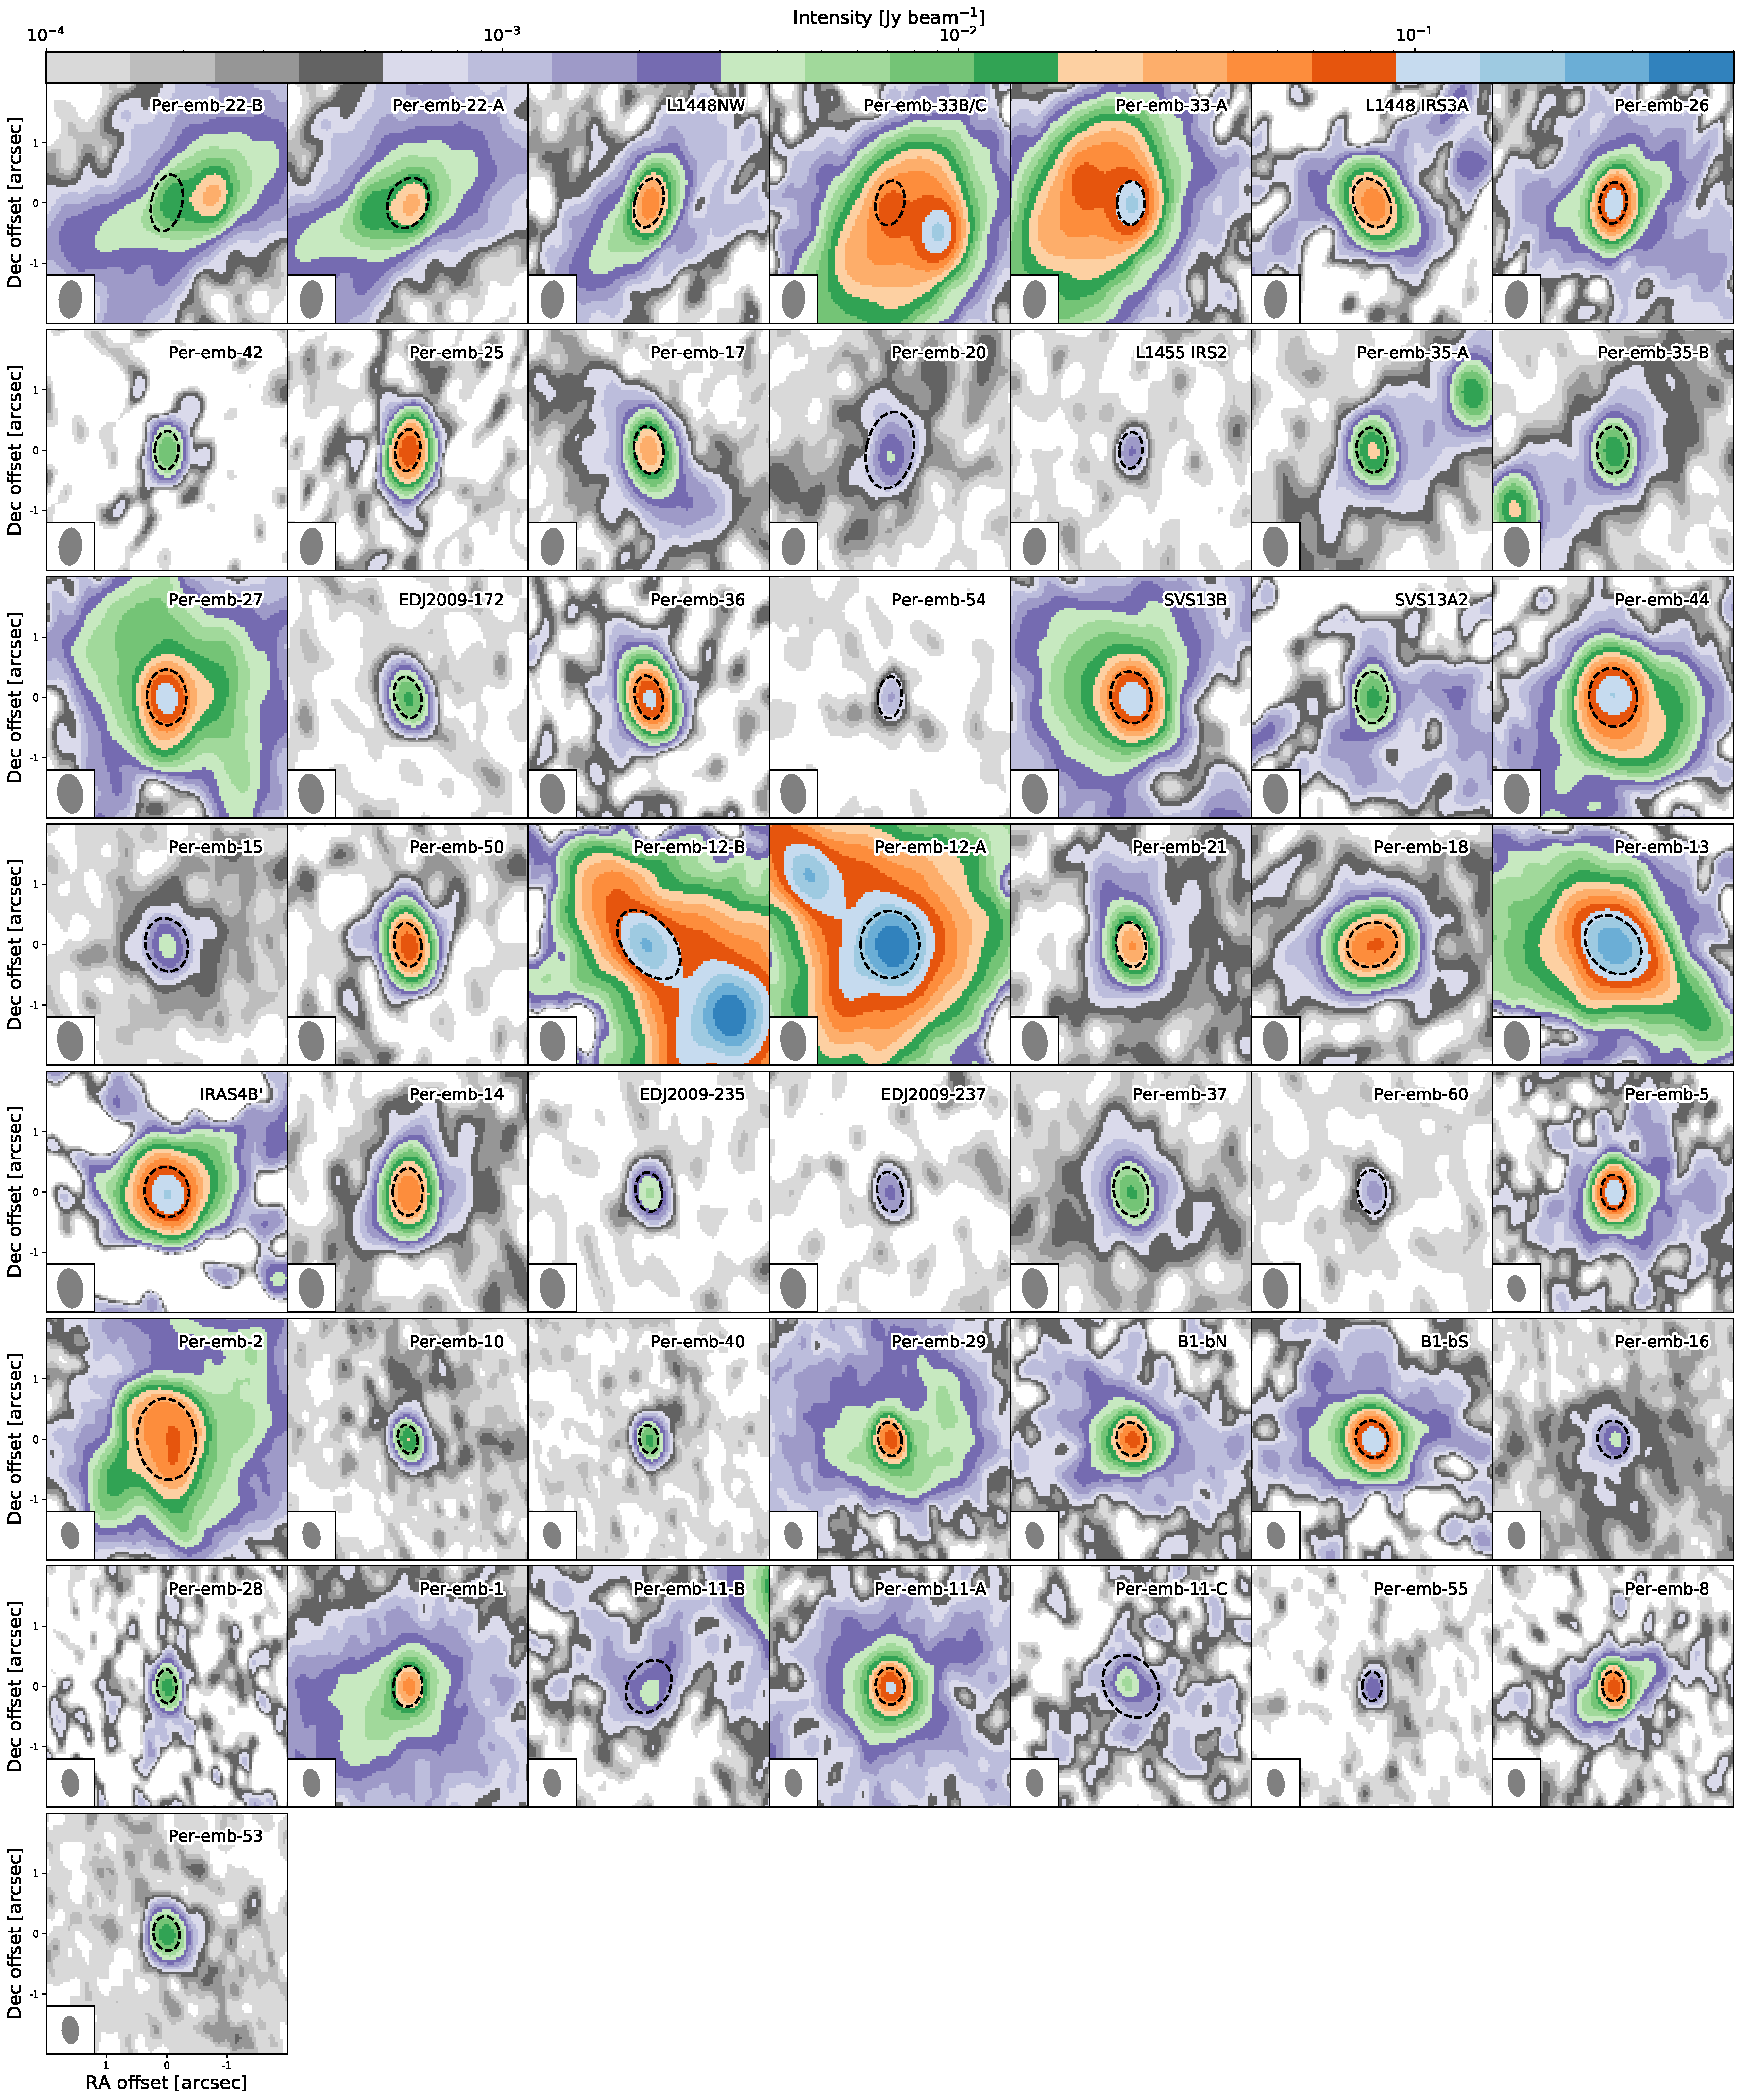
\includegraphics[width=\textwidth]{all_continuum.pdf}
  \caption{The continuum images of all PEACHES protostars.  Non-detections toward L1448 IRS\,2E and NGC 1333 SVS 3 are not shown.  The dashed ellipses illustrate the size of fitted continuum, which is the region for extracting 1D spectra.}
  \label{fig:continuum}
\end{figure*}

Three sources, EDJ2009-237, Per-emb-60, and EDJ2009-172, have no spectral line detected; therefore, we exclude them from spectral extraction as well as the line identification and modeling.  \textcolor{red}{These threee sources still need to be included for detection number statistics.}

\subsection{Line Identifications and Modeling}
\label{sec:modeling}
Line identification starts with manual identification and verification for a few sources with rich spectra, including Per-emb-12B and B1-bS.  We use \textsc{splatalogue}\footnote{\href{http://www.splatalogue.net/}{http://www.splatalogue.net/}} to identity the molecular species and use \textsc{xclass} \citep{2017A&A...598A...7M} to verify the identification.  The \textsc{xclass} package is a LTE radiative transfer code that uses the molecular data from the Cologne Database of Molecular Spectroscopy (CDMS; \citealt{2001A&A...370L..49M,2005JMoSt.742..215M,2016JMoSp.327...95E}) and the Jet Propulsion Laboratory (JPL; \citealt{1998JQSRT..60..883P}).  An identification needs to satisfy the following criteria.
\begin{itemize}
  \item The spectra agree with the predicted strengths of the model.
  \item The spectral lines are not all blended with other emission, such as other molecules and the SiO emission tracing the outflows.  The emission of a few species, such as HDCO \&\ \tmethanol, \acetaldehyde\ \&\ \dmethanol, $^{34}$SO \&\ \ethanol, and \dimethylether\ \&\ \dmethylcyanide, are partially blended (blending occurs at a few lines but other lines remain isolated).  The fittings of those species are performed together to verify their identification.
  \item Identified molecules need to be already found toward young stellar objects as summarized in \citet{2018ApJS..239...17M}. 
\end{itemize}
Table\,\ref{tbl:line_id} lists the identified species and transitions.  Only identifiable transitions are listed.  The \textsc{xclass} modeling includes all the transitions in our frequency coverage regardless their Einstein-A values and upper energy levels.  

Systematic spectral fitting using \textsc{xclass} is then applied to all sources using a list of species, compiled from those identifications.  The catalogs used in this study are listed in Appendix\,\ref{sec:catalogs}  The fitting function in \textsc{xclass} includes several optimization algorithms that can be used in series to reduce biases.  We configure the algorithm chain that starts with the genetic algorithm followed by the Levenberg-Marquardt $\chi^{2}$ minimization.  The genetic algorithm searches the best-fitting parameters iteratively with generations that evolve like a natural selection, where the better fitting models get less modification over generations.  We setup the genetic algorithm to search for the three best-fitting models after five generations.  Then, the Levenberg-Marquardt $\chi^{2}$ minimization applies to the three best-fitting models for 50 iterations to the best-fitting models.  We assume the COMs are all concentrated at the center, simplified as a 2D thin circular disk.  There are four parameters for the \textsc{xclass} modeling, the size of the emitting molecule ($r_\text{COM}$), the excitation temperature ($T_\text{ex}$), the column density ($N_\text{COM}$), and the line width ($\Delta \nu$).  Due to the limited frequency coverage, many species only have a few lines detected, we fix $r_\text{COM}$ as 0\farcs{5}, similar to our beam size, and optimize the model with five excitation temperatures, 100, 150, 200, 250, and 300 K.  We allow the line width varying between 1.2\,\kms\ to 3.5\,\kms\ for better fitting quality, and the range of the column density for each molecule is chosen according to the strength of the emission.  The range of fitted column densities at different temperatures indicates the uncertainty of the column densities.

The uncertainty from the fitting.

\newpage
\startlongtable
\begin{deluxetable*}{cccccc}
    \tabletypesize{\scriptsize}
    \tablecaption{Line Identification \label{tbl:line_id}}
    \tablewidth{\textwidth}
    \tablehead{\colhead{Frequency (MHz)} & \colhead{Transition\tablenotemark{a}} & 
               \colhead{log(Einstein-A)} & \colhead{$E_\text{u}$ (K)} & \colhead{$g_\text{u}$} & \colhead{Ref.}}
    \startdata
    \multicolumn{6}{c}{Ethynyl (CCH)} \\
    \hline
    262065.00 (0.05) & [3, 5/2, 3]\rt[2, 3/2, 2]\tablenotemark{b}   & $-$4.31 & 25.16  & 7  & CDMS \\
    262067.47 (0.05) & [3, 5/2, 2]\rt[2, 3/2, 1]\tablenotemark{b}   & $-$4.35 & 25.16  & 5  & CDMS \\
    262078.93 (0.02) & [3, 5/2, 2]\rt[2, 3/2, 2]\tablenotemark{b}   & $-$5.22 & 25.16  & 5  & CDMS \\
    \hline
    \multicolumn{6}{c}{Cyclopropenylidene (\cctht)} \\
    \hline
    244222.15 (0.01) & [3, 2, 1]\rt[2, 1, 2]                        & $-$4.23 & 18.17  & 21 & CDMS \\
    246557.77 (0.02) & [16, 10, 7]\rt[16, 9, 8]                     & $-$3.36 & 397.83 & 99 & CDMS \\
    260479.75 (0.02) & [5, 3, 2]\rt[4, 4, 1]                        & $-$3.79 & 44.72  & 33 & CDMS \\
    \hline
    \multicolumn{6}{c}{Methanol (\methanol\ $v_\text{t}=0$)} \\
    \hline
    243915.79 (0.01) & [5, 1, 4]\rt[4, 1, 3] A                      & $-$4.22 & 49.66  & 44 & CDMS \\
    246074.61 (0.02) & [20, 3, 17]\rt[20, 2, 18] A                  & $-$4.08 & 537.03 & 164& CDMS \\
    246873.30 (0.02) & [19, 3, 16]\rt[19, 2, 17] A                  & $-$4.08 & 490.65 & 156& CDMS \\
    261805.68 (0.01) & [2, 1, 1]\rt[1, 0, 1] E                      & $-$4.25 & 28.01  & 20 & CDMS \\
    \hline
    \multicolumn{6}{c}{Methanol (\tmethanol\ $v_\text{t}=0$)} \\
    \hline
    246426.12 (0.22) & [23, 4, 19]\rt[22, 5, 18]                    & $-$4.58 & 721.02 & 47 & CDMS \\
    247086.3 (0.5)   & [23, 3, 20]\rt[23, 2, 21] A$-$\rt\ A$+$      & $-$4.07 & 674.86 & 47 & CDMS \\
    259036.49 (0.17) & [17, 3, 15]\rt[17, 2, 16] A$+$\rt\ A$-$      & $-$4.04 & 396.48 & 35 & CDMS \\
    \hline
    \multicolumn{6}{c}{Methanol (\dmethanol\ $v_\text{t}=0$)} \\
    \hline
    243514.31 (0.01) & [9, 2, 8]\rt[10, 1, 10] o$_\text{1}$         & $-$5.17 & 131.85 & 19 & JPL  \\
    246973.11 (0.01) & [4, 1, 4]\rt[4, 1, 3] e$_\text{1}$           & $-$4.67 & 37.69  & 9  & JPL  \\
    260543.63 (0.01) & [3, 2, 1]\rt[3, 1, 2] o$_\text{1}$           & $-$4.65 & 48.34  & 7  & JPL  \\
    \hline
    \multicolumn{6}{c}{Methanol (\etmethanol\ $v_\text{t}=0$)} \\
    \hline
    246256.60 (0.04) & [11. 2. 10]\rt[10, 3, 7] A                   & $-$4.64 & 184.27 & 92 & CDMS \\
    \hline
    \multicolumn{6}{c}{Sulfur monoxide (\sosigma)} \\
    \hline
    258255.83 (0.01) & [\N, \J]$=$[6, 6]\rt[5, 5]                   & $-$3.67 & 56.50  & 13 & CDMS \\
    261843.72 (0.03) & [\N, \J]$=$[7, 6]\rt[6, 5]                   & $-$3.64 & 47.55  & 15 & CDMS \\
    \hline
    \multicolumn{6}{c}{Sulfur monoxide (\tfso)} \\
    \hline
    246663.47 (0.1)  & [\N, \J]$=$[5, 6]\rt[4, 5]                   & $-$3.74 & 49.89  & 11 & CDMS \\
    \hline
    \multicolumn{6}{c}{Sulfur dioxide (\sotwo)} \\
    \hline
    244254.22 (0.01) & [14, 0, 14]\rt[13, 1, 13]                    & $-$3.79 & 93.90  & 29 & CDMS \\
    \hline
    \multicolumn{6}{c}{Hydrogen cyanide (\htcn)} \\
    \hline
    259010.26 (0.01) & [\J, \F]$=$[3, 3]\rt[2, 3]                   & $-$4.07 & 24.86  & 7  & CDMS \\
    259011.55 (0.01) & [\J, \F]$=$[3, 2]\rt[2, 1]                   & $-$3.19 & 24.86  & 5  & CDMS \\
    259011.80 (0.01) & [\J, \F]$=$[3, 3]\rt[2, 2]                   & $-$3.16 & 24.86  & 7  & CDMS \\
    259011.86 (0.01) & [\J, \F]$=$[3, 4]\rt[2, 3]                   & $-$3.11 & 24.86  & 9  & CDMS \\
    259012.34 (0.01) & [\J, \F]$=$[3, 2]\rt[2, 3]                   & $-$5.46 & 24.86  & 5  & CDMS \\
    259013.89 (0.01) & [\J, \F]$=$[3, 2]\rt[2, 2]                   & $-$3.92 & 24.86  & 5  & CDMS \\
    \hline
    \multicolumn{6}{c}{Carbon Monosulfide (CS)} \\
    \hline
    244935.56 (0.01) & [\J]$=$[5]\rt[4]                             & $-$3.53 & 35.27  & 11 & CDMS \\
    \hline
    \multicolumn{6}{c}{Formaldehyde (HDCO)} \\
    \hline
    246924.6 (0.1)   & [4, 1, 4]\rt[3, 1, 3]                        & $-$3.40 & 37.60  & 9  & CDMS \\
    259034.9 (0.1)   & [4, 2, 2]\rt[3, 2, 1]                        & $-$3.44 & 62.86  & 9  & CDMS \\
    \hline
    \multicolumn{6}{c}{Methyl formate (\methylformate)} \\
    \hline
    245883.2 (0.1)   & [20, 13, 7]\rt[19, 13, 6] E                  & $-$3.89 & 235.98 & 82 & JPL  \\
    245885.2 (0.1)   & [20, 13, 7]\rt[19, 13, 6] A                  & $-$3.89 & 235.98 & 82 & JPL  \\
    245885.2 (0.1)   & [20, 13, 8]\rt[19, 13, 7] A                  & $-$3.89 & 235.98 & 82 & JPL  \\
    245903.7 (0.1)   & [20, 13, 8]\rt[19, 13, 7] E                  & $-$3.89 & 235.97 & 82 & JPL  \\
    246027.5 (0.1)   & [21, 2, 19]\rt[20, 3, 18] E                  & $-$4.63 & 139.85 & 86 & JPL  \\
    246038.9 (0.1)   & [21, 2, 19]\rt[20, 3, 18] A                  & $-$4.63 & 139.85 & 86 & JPL  \\
    246054.8 (0.1)   & [20, 12, 8]\rt[19, 12, 7] E                  & $-$3.84 & 219.43 & 82 & JPL  \\
    246060.8 (0.1)   & [20, 12, 8/9]\rt[19, 12, 7/8] A              & $-$3.84 & 219.43 & 82 & JPL  \\
    246076.9 (0.1)   & [20, 12, 9]\rt[19, 12, 8] E                  & $-$3.84 & 219.41 & 82 & JPL  \\
    246285.4 (0.1)   & [20, 11, 9]\rt[19, 11, 8] E                  & $-$3.80 & 204.21 & 82 & JPL  \\
    246295.1 (0.1)   & [20, 11, 10]\rt[19, 11, 9] A                 & $-$3.80 & 204.21 & 82 & JPL  \\
    246295.1 (0.1)   & [20, 11, 9]\rt[19, 11, 8] A                  & $-$3.80 & 204.21 & 82 & JPL  \\
    246308.3 (0.1)   & [20, 11, 10]\rt[19, 11, 9] E                 & $-$3.80 & 204.20 & 82 & JPL  \\
    246456.1 (0.1)   & [10, 5, 6]\rt[9, 4, 5] E                     & $-$5.52 & 49.09  & 42 & JPL  \\
    246600.0 (0.1)   & [20, 10, 10]\rt[19, 10, 9] E                 & $-$3.77 & 190.34 & 82 & JPL  \\
    246613.4 (0.1)   & [20, 10, 11]\rt[19, 10, 10] A                & $-$3.77 & 190.34 & 82 & JPL  \\
    246613.4 (0.1)   & [20, 10, 10]\rt[19, 10, 9] A                 & $-$3.77 & 190.34 & 82 & JPL  \\
    246623.2 (0.1)   & [20, 10, 11]\rt[19, 10, 10] E                & $-$3.77 & 190.34 & 82 & JPL  \\
    % 246630.0 (0.1)   & [35, 6, 30]\rt[35, 5, 31] A                  & $-$4.77 & 397.98 &142 & JPL  \\
    246660.5 (0.1)   & [10, 5, 6]\rt[9, 4, 5] A                     & $-$4.74 & 49.08  & 42 & JPL  \\
    246675.4 (0.1)   & [15, 4, 12]\rt[14, 3, 11] E                  & $-$4.93 & 81.85  & 62 & JPL  \\
    246683.5 (0.1)   & [15, 4, 12]\rt[14, 3, 11] A                  & $-$4.93 & 81.84  & 62 & JPL  \\
    246752.9 (0.1)   & [10, 5, 5]\rt[9, 4, 5] E                     & $-$4.90 & 49.10  & 42 & JPL  \\
    246891.6 (0.1)   & [19, 4, 15]\rt[18, 4, 14] E                  & $-$3.66 & 126.22 & 78 & JPL  \\
    246914.7 (0.1)   & [19, 4, 15]\rt[18, 4, 14] A                  & $-$3.66 & 126.22 & 78 & JPL  \\
    246945.7 (0.1)   & [10, 5, 6]\rt[9, 4, 6] E                     & $-$4.90 & 49.09  & 42 & JPL  \\
    247040.7 (0.1)   & [20, 9, 11]\rt[19, 9, 10] E                  & $-$3.74 & 177.83 & 82 & JPL  \\
    247044.1 (0.1)   & [21, 3, 19]\rt[20, 3, 18] E                  & $-$3.66 & 139.90 & 86 & JPL  \\
    247053.5 (0.1)   & [21, 3, 19]\rt[20, 3, 18] A                  & $-$3.66 & 139.89 & 86 & JPL  \\
    247057.3 (0.1)   & [20, 9, 12]\rt[19, 9, 11] A                  & $-$3.74 & 177.83 & 82 & JPL  \\
    247057.7 (0.1)   & [20, 9, 11]\rt[19, 9, 10] A                  & $-$3.74 & 177.83 & 82 & JPL  \\
    247063.7 (0.1)   & [20, 9, 12]\rt[19, 9, 11] E                  & $-$3.74 & 177.83 & 82 & JPL  \\
    247124.3 (0.1)   & [10, 5, 5]\rt[9, 4, 6] E                     & $-$4.74 & 49.08  & 42 & JPL  \\
    258275.0 (0.1)   & [21, 13, 8]\rt[20, 13, 7] E                  & $-$3.79 & 248.37 & 86 & JPL  \\
    258277.4 (0.1)   & [21, 13, 8]\rt[20, 13, 7] A                  & $-$3.79 & 248.37 & 86 & JPL  \\
    258277.4 (0.1)   & [21, 13, 9]\rt[20, 13, 8] A                  & $-$3.79 & 248.37 & 86 & JPL  \\
    259341.9 (0.1)   & [24, 0, 24]\rt[23, 1, 23] E                  & $-$4.37 & 158.23 & 98 & JPL  \\
    259342.0 (0.1)   & [24, 1, 24]\rt[23, 1, 23] E                  & $-$3.58 & 158.23 & 98 & JPL  \\
    259342.1 (0.1)   & [24, 0, 24]\rt[23, 0, 23] E                  & $-$3.58 & 158.23 & 98 & JPL  \\
    259342.3 (0.1)   & [24, 1, 24]\rt[23, 0, 23] E                  & $-$4.37 & 158.23 & 98 & JPL  \\
    259342.7 (0.1)   & [24, 0, 24]\rt[23, 1, 23] A                  & $-$4.37 & 158.22 & 98 & JPL  \\
    259342.9 (0.1)   & [24, 1, 24]\rt[23, 1, 23] A                  & $-$3.58 & 158.22 & 98 & JPL  \\
    259343.0 (0.1)   & [24, 0, 24]\rt[23, 0, 23] A                  & $-$3.58 & 158.22 & 98 & JPL  \\
    259343.2 (0.1)   & [24, 1, 24]\rt[23, 0, 23] A                  & $-$4.37 & 158.22 & 98 & JPL  \\
    261822.3 (0.1)   & [17, 10, 7]\rt[17, 9, 8] A                   & $-$4.73 & 156.63 & 70 & JPL  \\
    262088.2 (0.1)   & [16, 10, 6]\rt[16, 9, 7] A                   & $-$4.76 & 146.59 & 66 & JPL  \\
    262088.2 (0.1)   & [16, 10, 7]\rt[16, 9, 8] A                   & $-$4.76 & 146.59 & 66 & JPL  \\
    \hline
    \multicolumn{6}{c}{Methyl formate (\methylformatev)} \\
    \hline
    243511.5 (0.1)   & [20, 12, 8]\rt[19, 12, 7] E                  & $-$3.85 & 407.25 & 82 & JPL  \\
    245846.9 (0.1)   & [21, 3, 19]\rt[20, 3, 18] E                  & $-$3.66 & 326.30 & 86 & JPL  \\
    246106.8 (0.1)   & [20, 7, 14]\rt[19, 7, 13] A                  & $-$3.70 & 343.77 & 82 & JPL  \\
    246184.2 (0.1)   & [20, 8, 13]\rt[19, 8, 12] E                  & $-$3.72 & 353.27 & 82 & JPL  \\
    246187.0 (0.1)   & [21, 2, 19]\rt[20, 2, 18] A                  & $-$3.66 & 326.62 & 86 & JPL  \\
    246233.6 (0.1)   & [20, 7, 13]\rt[19, 7, 12] A                  & $-$3.70 & 343.79 & 82 & JPL  \\
    246274.9 (0.1)   & [20, 7, 13]\rt[19, 7, 12] E                  & $-$3.70 & 343.86 & 82 & JPL  \\
    246410.95 (0.01) & [10, 5, 5]\rt[9, 4, 6] A                     & $-$4.73 & 236.70 & 42 & JPL  \\
    246422.7 (0.1)   & [22, 1, 21]\rt[21, 2, 20] A                  & $-$4.51 & 330.43 & 90 & JPL  \\
    246461.2 (0.1)   & [22, 2, 21]\rt[21, 2, 20] A                  & $-$3.65 & 330.43 & 90 & JPL  \\
    246488.4 (0.1)   & [22, 1, 21]\rt[21, 1, 20] A                  & $-$3.65 & 330.43 & 90 & JPL  \\
    246562.9 (0.1)   & [21, 2, 19]\rt[20, 2, 18] E                  & $-$3.66 & 326.24 & 86 & JPL  \\
    246706.5 (0.1)   & [22, 2, 21]\rt[21, 2, 20] E                  & $-$3.65 & 329.89 & 90 & JPL  \\
    246731.7 (0.1)   & [22, 1, 21]\rt[21, 1, 20] E                  & $-$3.65 & 329.89 & 90 & JPL  \\
    246985.2 (0.1)   & [20, 6, 15]\rt[19, 6, 14] A                  & $-$3.68 & 335.37 & 82 & JPL  \\
    259003.9 (0.1)   & [21, 7, 14]\rt[20, 7, 13] A                  & $-$3.63 & 356.22 & 86 & JPL  \\
    259025.8 (0.1)   & [21, 7, 14]\rt[20, 7, 13] E                  & $-$3.63 & 356.29 & 86 & JPL  \\
    260479.6 (0.1)   & [44, 9, 36]\rt[44, 8, 37] A                  & $-$4.59 & 828.74 & 178& JPL  \\
    \hline
    \multicolumn{6}{c}{Dimethyl ether (\dimethylether)} \\
    \hline
    246499.29 (0.01) & [37, 6, 31]\rt[37, 5, 12] AA                 & $-$4.01 & 693.72 & 750& CDMS \\
    246505.09 (0.01) & [37, 6, 31]\rt[37, 5, 12] AE                 & $-$4.01 & 693.72 & 450& CDMS \\
    246505.09 (0.01) & [37, 6, 31]\rt[37, 5, 12] EA                 & $-$4.01 & 693.72 & 300& CDMS \\
    246697.43 (0.01) & [27, 4, 23]\rt[26, 5, 21] AA                 & $-$4.70 & 367.61 & 330& CDMS \\
    246697.87 (0.01) & [27, 4, 23]\rt[26, 5, 21] EE                 & $-$4.70 & 367.61 & 880& CDMS \\
    246698.31 (0.01) & [27, 4, 23]\rt[26, 5, 21] AE                 & $-$4.70 & 367.61 & 110& CDMS \\
    246698.31 (0.01) & [27, 4, 23]\rt[26, 5, 21] EA                 & $-$4.70 & 367.61 & 220& CDMS \\
    259305.22 (0.01) & [33, 3, 31]\rt[34, 6, 28] AA                 & $-$6.61 & 563.02 & 670& CDMS \\
    259308.39 (0.01) & [33, 3, 31]\rt[34, 6, 28] AE                 & $-$6.61 & 563.02 & 402& CDMS \\
    259308.39 (0.01) & [33, 3, 31]\rt[34, 6, 28] EA                 & $-$6.61 & 563.02 & 268& CDMS \\
    259309.47 (0.01) & [17, 5, 12]\rt[17, 4, 13] AE                 & $-$4.06 & 174.54 & 210& CDMS \\
    259309.76 (0.01) & [17, 5, 12]\rt[17, 4, 13] EA                 & $-$4.06 & 174.54 & 140& CDMS \\
    259311.95 (0.01) & [17, 5, 12]\rt[17, 4, 13] EE                 & $-$4.06 & 174.54 & 560& CDMS \\
    259314.28 (0.01) & [17, 5, 12]\rt[17, 4, 13] AA                 & $-$4.06 & 174.54 & 350& CDMS \\
    \hline
    \multicolumn{6}{c}{Acetone (\acetone)} \\
    \hline
    244218.91 (0.01) & [20, 5, 15]\rt[19, 6, 14] AE                 & $-$3.32 & 139.69 & 82 & JPL \\
    244218.91 (0.01) & [20, 6, 15]\rt[19, 5, 14] AE                 & $-$3.32 & 139.69 & 250& JPL \\
    244218.92 (0.01) & [20, 5, 15]\rt[19, 6, 14] EA                 & $-$3.32 & 139.69 & 160& JPL \\
    244218.92 (0.01) & [20, 6, 15]\rt[19, 5, 14] EA                 & $-$3.32 & 139.69 & 160& JPL \\
    245831.34 (0.09) & [13, 10, 3]\rt[12, 9, 4] EE                  & $-$3.80 & 77.84  & 432& JPL \\ 
    246400.99 (0.05) & [34, 7, 28]\rt[34, 5, 29] EE                 & $-$4.17 & 364.98 &1100& JPL \\
    246400.99 (0.05) & [34, 6, 28]\rt[34, 5, 29] EE                 & $-$4.03 & 364.98 &1100& JPL \\
    246400.99 (0.05) & [34, 7, 28]\rt[34, 6, 29] EE                 & $-$4.03 & 364.98 &1100& JPL \\
    246400.99 (0.05) & [34, 6, 28]\rt[34, 6, 29] EE                 & $-$4.17 & 364.98 &1100& JPL \\
    246404.27 (0.01) & [22, 3, 19]\rt[21, 4, 18] AE                 & $-$3.23 & 149.62 & 90 & JPL \\
    246404.27 (0.01) & [22, 4, 19]\rt[21, 3, 18] AE                 & $-$3.23 & 149.62 & 270& JPL \\
    246404.29 (0.01) & [22, 3, 19]\rt[21, 4, 18] EA                 & $-$3.23 & 149.62 & 180& JPL \\
    246404.29 (0.01) & [22, 4, 19]\rt[21, 3, 18] EA                 & $-$3.23 & 149.62 & 180& JPL \\
    246450.40 (0.01) & [22, 4, 19]\rt[21, 3, 18] EE                 & $-$3.23 & 149.57 & 720& JPL \\
    246450.40 (0.01) & [22, 3, 19]\rt[21, 3, 18] EE                 & $-$5.09 & 149.57 & 720& JPL \\
    246450.40 (0.01) & [22, 3, 19]\rt[21, 4, 18] EE                 & $-$3.24 & 149.57 & 720& JPL \\
    246450.40 (0.01) & [22, 4, 19]\rt[21, 4, 18] EE                 & $-$4.92 & 149.57 & 720& JPL \\
    246496.17 (0.46) & [25, 14, 12]\rt[24, 15, 9] AE                & $-$5.01 & 257.11 & 100& JPL \\
    246496.47 (0.02) & [22, 3, 19]\rt[21, 4, 18] AA                 & $-$3.23 & 149.51 & 270& JPL \\
    246496.47 (0.02) & [22, 4, 19]\rt[21, 3, 18] AA                 & $-$3.23 & 149.51 & 450& JPL \\
    246714.12 (0.05) & [9, 8, 1]\rt[8, 5, 4] EA                     & $-$5.84 & 40.59  & 76 & JPL \\
    246714.94 (0.05) & [32, 4, 28]\rt[32, 4, 29] EA                 & $-$3.97 & 305.61 & 260& JPL \\
    246714.94 (0.05) & [32, 5, 28]\rt[32, 3, 29] EA                 & $-$3.97 & 305.61 & 260& JPL \\
    246715.04 (0.05) & [32, 5, 28]\rt[32, 4, 29] AE                 & $-$3.97 & 305.61 & 390& JPL \\
    246715.04 (0.05) & [32, 4, 28]\rt[32, 3, 29] EA                 & $-$3.97 & 305.61 & 130& JPL \\
    246719.92 (0.04) & [33, 6, 28]\rt[33, 4, 29] EE                 & $-$5.62 & 344.85 &1100& JPL \\
    246719.92 (0.04) & [33, 5, 28]\rt[33, 4, 29] EE                 & $-$3.87 & 344.85 &1100& JPL \\
    246719.92 (0.04) & [33, 6, 28]\rt[33, 5, 29] EE                 & $-$3.87 & 344.85 &1100& JPL \\
    246719.92 (0.04) & [33, 5, 28]\rt[33, 5, 29] EE                 & $-$5.61 & 344.85 &1100& JPL \\
    261818.11 (0.01) & [20, 7, 13]\rt[19, 8, 12] EA                 & $-$3.31 & 151.17 & 160& JPL \\
    261818.17 (0.01) & [20, 7, 13]\rt[19, 8, 12] AE                 & $-$3.31 & 151.17 & 82 & JPL \\
    261819.09 (0.01) & [20, 8, 13]\rt[19, 7, 12] EA                 & $-$3.31 & 151.17 & 160& JPL \\
    261819.17 (0.01) & [20, 8, 13]\rt[19, 7, 12] AE                 & $-$3.31 & 151.17 & 250& JPL \\
    \hline
    \multicolumn{6}{c}{Methyl cyanide (\methylcyanide)} \\
    \hline
    257507.56 (0.01) & [\N, \K]$=$[14, 2]\rt[13, 2]                 & $-$3.00 & 121.28 & 58 & JPL \\
    257522.43 (0.01) & [\N, \K]$=$[14, 1]\rt[13, 1]                 & $-$2.99 & 99.84  & 58 & JPL \\
    257527.38 (0.01) & [\N, \K]$=$[14, 0]\rt[13, 0]                 & $-$2.99 & 92.70  & 58 & JPL \\
    \hline
    \multicolumn{6}{c}{Acetaldehyde (\acetaldehyde\ $v_\text{t}=0$)} \\
    \hline
    246330.73 (0.01) & [15, 3, 13]\rt[15, 2, 14] A                  & $-$4.29 & 131.49 & 62 & JPL \\
    260530.40 (0.01) & [14, 1, 14]\rt[13, 1, 13] E                  & $-$3.20 & 96.39  & 58 & JPL \\
    260544.02 (0.01) & [14, 1, 14]\rt[13, 1, 13] A                  & $-$3.20 & 96.32  & 58 & JPL \\
    260547.46 (2.07) & [9, 4, 5]\rt[9, 3, 7] E, $v_\text{t}=2$      & $-$6.06 & 456.38 & 38 & JPL \\
    \hline
    \multicolumn{6}{c}{gauche-Ethanol ($g$-\ethanol)} \\
    \hline
    246414.76 (0.05) & [14, 3, 11]\rt[13, 3, 10] $v_\text{t}=0$\rt0 & $-$3.89 & 155.72 & 29 & JPL \\
    246524.28 (0.01) & [13, 2, 12]\rt[12, 1, 12] $v_\text{t}=0$\rt1 & $-$4.50 & 136.95 & 27 & JPL \\
    246658.18 (0.01) & [32, 5, 28]\rt[32, 4, 29] $v_\text{t}=0$\rt0 & $-$6.33 & 527.94 & 65 & JPL \\
    246662.98 (0.01) & [4, 2, 3]\rt[3, 1, 3] $v_\text{t}=1$\rt0     & $-$4.36 & 74.77  & 9  & JPL \\
    259322.64 (0.01) & [14, 3, 11]\rt[13, 2, 11] $v_\text{t}=0$\rt1 & $-$4.39 & 155.72 & 29 & JPL \\
    260457.73 (0.01) & [15. 4. 12]\rt[14, 4, 11] $v_\text{t}=1$\rt1 & $-$3.83 & 181.10 & 31 & JPL \\
    \hline
    \multicolumn{6}{c}{trans-Ethanol (\ethanol)} \\
    \hline
    246663.62 (0.05) & [24, 1, 23]\rt[24, 0, 24]                    & $-$3.73 & 252.35 & 49 & JPL \\
    261815.99 (0.05) & [28, 3, 26]\rt[28, 2, 27]                    & $-$3.96 & 350.98 & 57 & JPL \\
    \hline
    \multicolumn{6}{c}{Glycolaldehyde ($cis$-\glycolaldehyde)} \\
    \hline
    246773.09 (0.02) & [30, 2, 28]\rt[30, 1, 29]                    & $-$4.04 & 252.68 & 61 & CDMS \\
    246778.28 (0.02) & [30, 3, 28]\rt[30, 2, 29]                    & $-$4.04 & 252.68 & 61 & CDMS \\
    262056.78 (0.01) & [25, 2, 24]\rt[24, 1, 23]                    & $-$3.34 & 158.25 & 51 & CDMS \\
    261795.48 (0.01) & [25, 11, 14]\rt[25, 10, 15]                  & $-$3.57 & 254.23 & 51 & CDMS \\
    261798.96 (0.01) & [25, 11, 15]\rt[25, 10, 16]                  & $-$3.57 & 254.23 & 51 & CDMS \\
    \hline
    \multicolumn{6}{c}{Methyl cyanide (\dmethylcyanide)} \\
    \hline
    259315.51 (0.01) & [15, 1, 15]\rt[14, 1, 14]                    & $-$2.82 & 104.97 & 31 & CDMS \\
    260523.05 (0.01) & [15, 2, 13]\rt[14, 2, 12]                    & $-$2.82 & 121.60 & 31 & CDMS \\
    \hline
    \multicolumn{6}{c}{Ethyl cyanide (\ethylcyanide)} \\
    \hline
    246268.74 (0.01) & [27, 2, 25]\rt[26, 2, 24]                    & $-$2.90 & 169.80 & 55 & CDMS \\
    246421.92 (0.01) & [28, 2, 27]\rt[27, 2, 26]                    & $-$2.90 & 177.26 & 57 & CDMS \\
    246548.70 (0.01) & [27, 3, 24]\rt[26, 3, 23]                    & $-$2.90 & 174.06 & 55 & CDMS \\
    260535.69 (0.05) & [29, 5, 25]\rt[28, 5, 24]                    & $-$2.84 & 215.06 & 59 & CDMS \\
    \hline
    \multicolumn{6}{c}{Formamide (\formamide)} \\
    \hline
    243521.04 (0.01) & [12, 1, 12]\rt[11, 1, 11]                    & $-$2.98 & 79.19  & 25 & CDMS \\
    \hline
    \multicolumn{6}{c}{Formic acid (\tcooh)} \\
    \hline
    262103.48 (0.01) & [12, 0, 12]\rt[11, 0, 11]                    & $-$3.69 & 82.77  & 25 & CDMS \\
    \enddata
    \tablenotetext{a}{The typical quantum numbers are listed as [\J, \Ka, \Kc] unless specified.}
    \tablenotetext{b}{The quantum numbers are [\N, \J, \F]}
\end{deluxetable*}

\section{Continuum Opacity}


\section{Detection Statistics}
We summarize the fraction of sources with detections of molecules in Figure\,\ref{fig:stats}.  The detection statistics include COMs, carbon-chain molecules, and the simple organic molecules, such as CS, \htcn, SO, $^{34}$SO, and SO$_{2}$.  The PEACHES protostars show a great chemical diversity from no molecule detected (\textcolor{red}{B1-bN}) to rich spectra of COMs (e.g. Per-emb-12B).  Detections of COMs and the number of COMs detected show no obvious correlation with the bolometric luminosity and bolometric temperature of the protostars, which are conventional evolutionary indicators.  Low luminosity sources have fewer COMs detected; however, if COMs mostly come from thermally desorption, the region with $T > T_\text{desorption}$ may be smaller for the low luminosity sources, making the emission of COMs fainter and reducing our sensitivity to detect COMs.  We also compare the detection statistics with the mass derived from 9\,mm observations that resolved the sources as a proxy of the central mass \citep{2018ApJS..238...19T}.  The detection statistics show no clear correlation with the central mass; however, the sources with smaller central mass have fewer detections of COMs, \textcolor{red}{which may due to their low luminosity.}  

\begin{figure*}[htbp!]
  \centering
  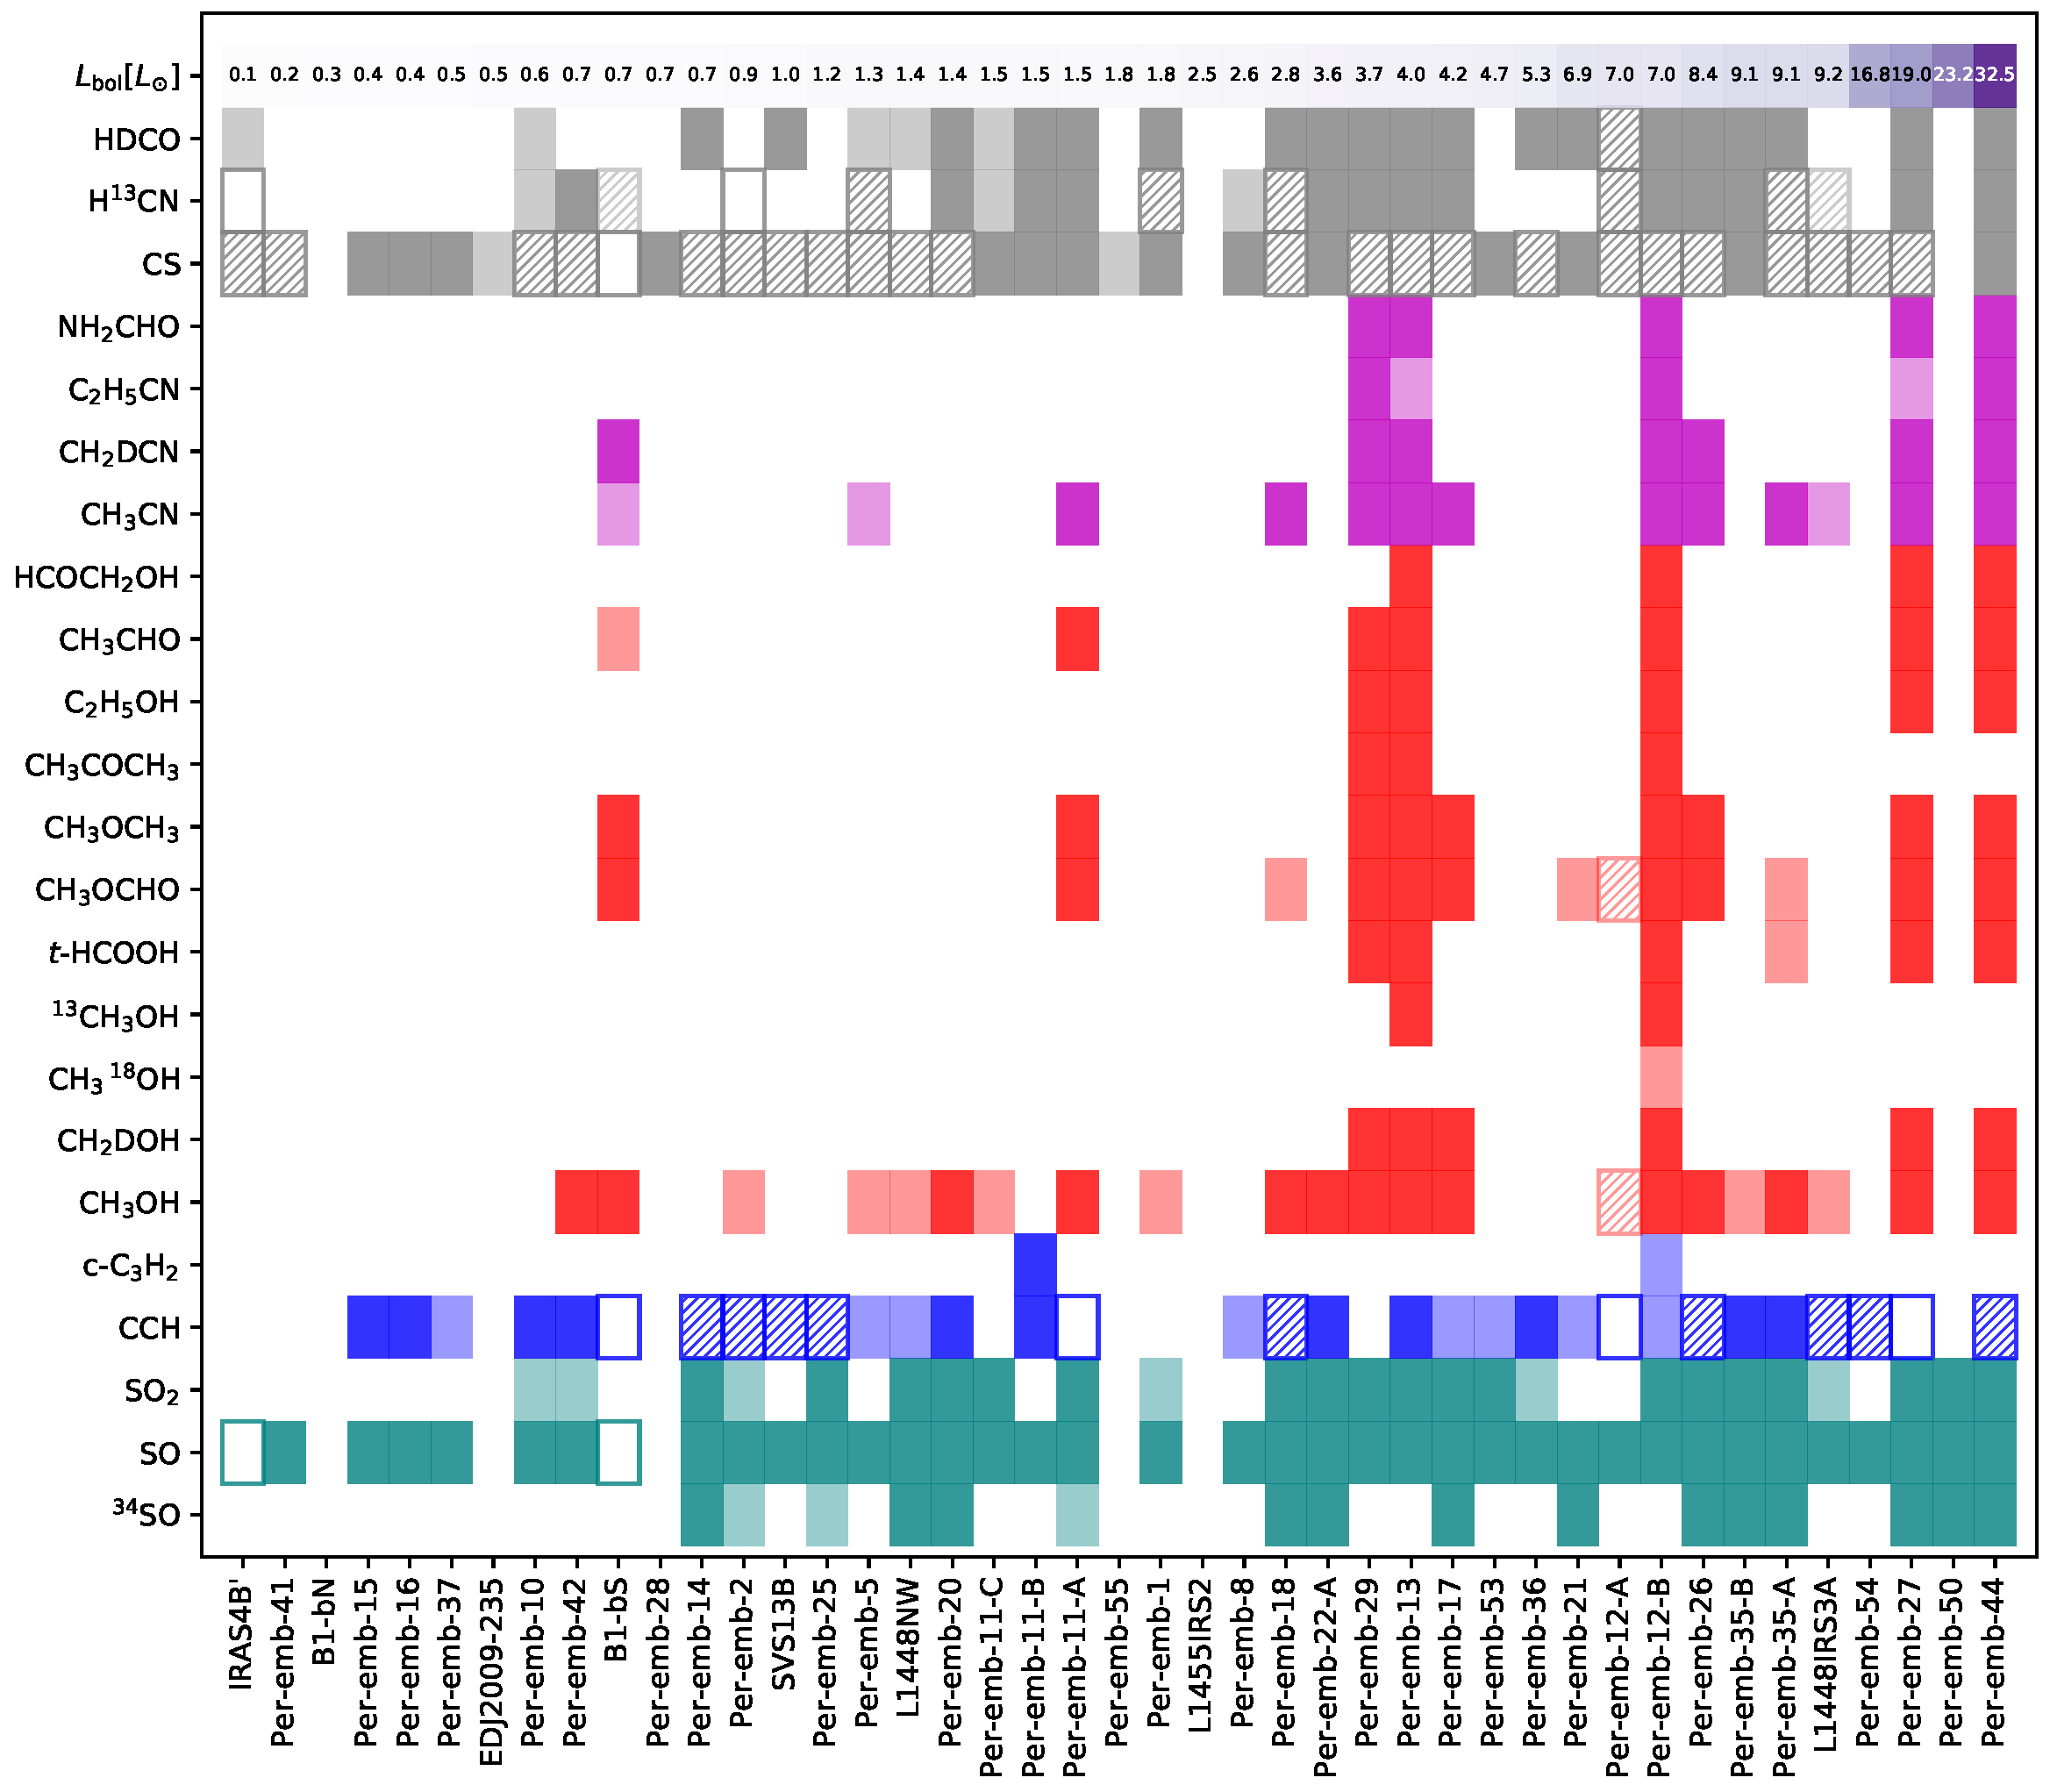
\includegraphics[width=\textwidth]{stats_sorted_by_lbol.pdf}
  \caption{The detection statistics sorted by their bolometric luminosity.}
  \label{fig:stats}
\end{figure*}

\renewcommand{\thefigure}{\arabic{figure} (Cont.)}
\addtocounter{figure}{-1}
\begin{figure*}[htbp!]
  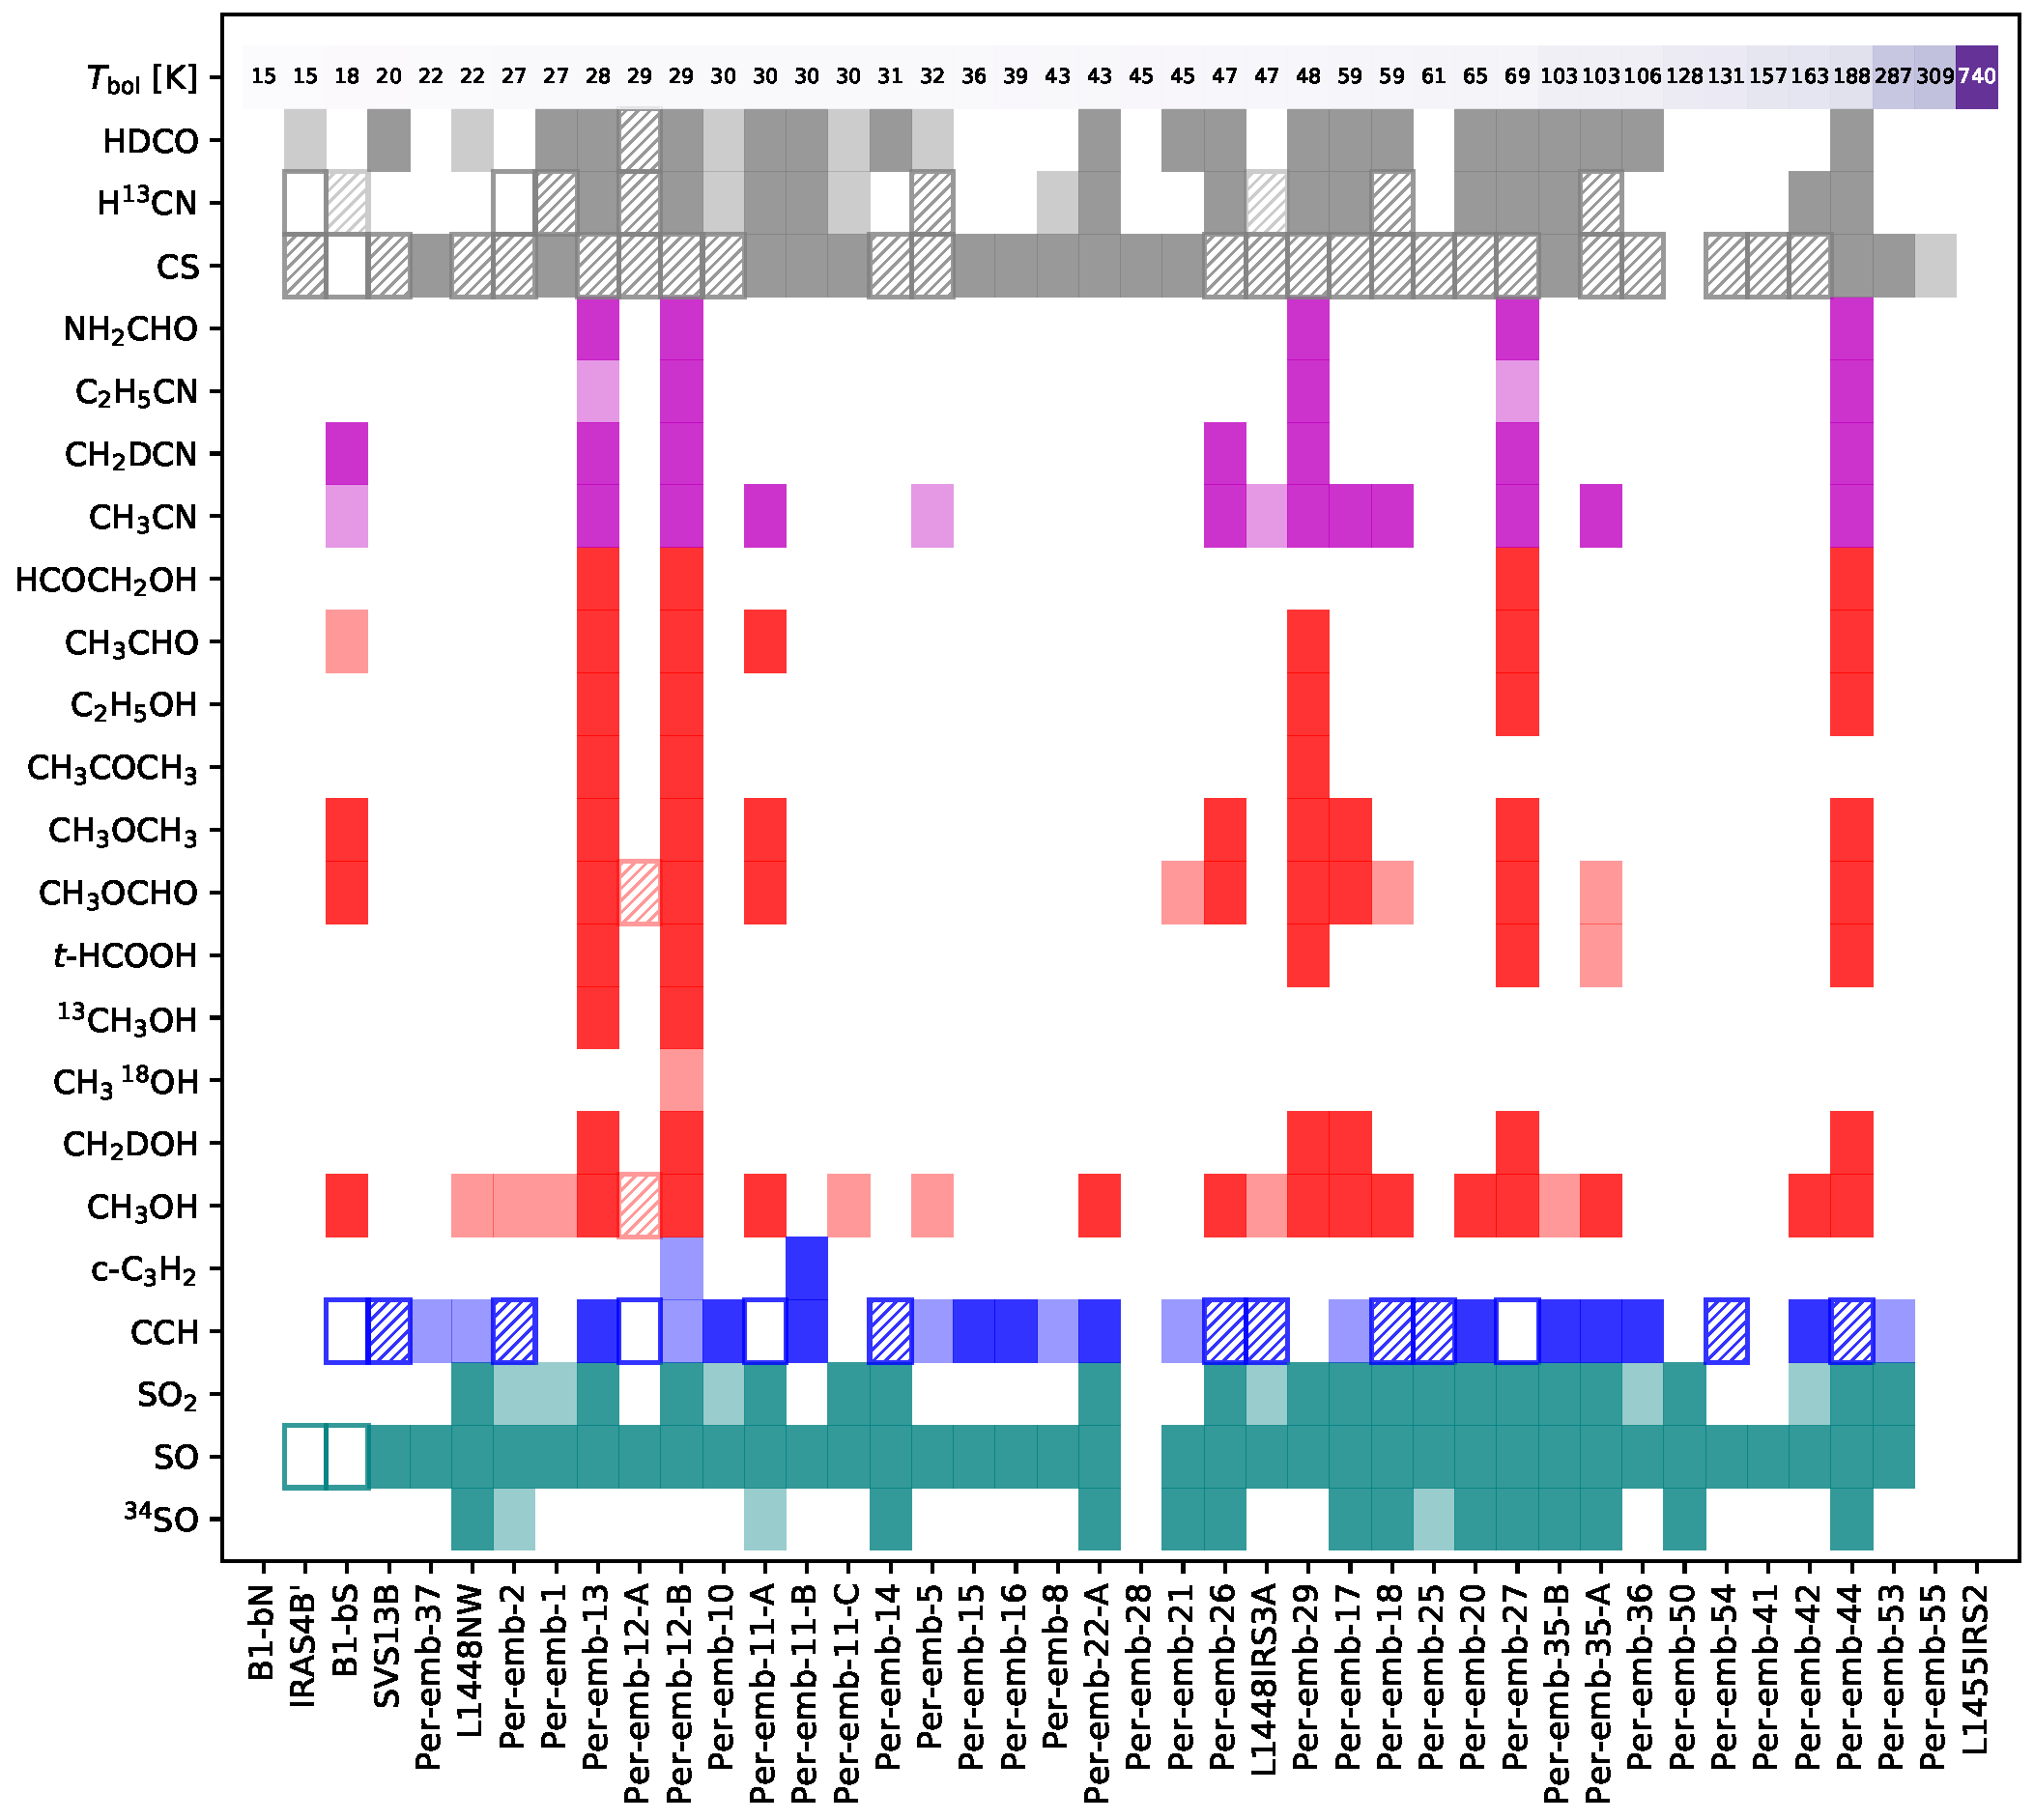
\includegraphics[width=\textwidth]{stats_sorted_by_tbol.pdf}
  \caption{The same figure as Figure\,\ref{fig:stats} but sorted by their bolometric temperature.}
\end{figure*}
\addtocounter{figure}{-1}

\begin{figure*}[htbp!]
  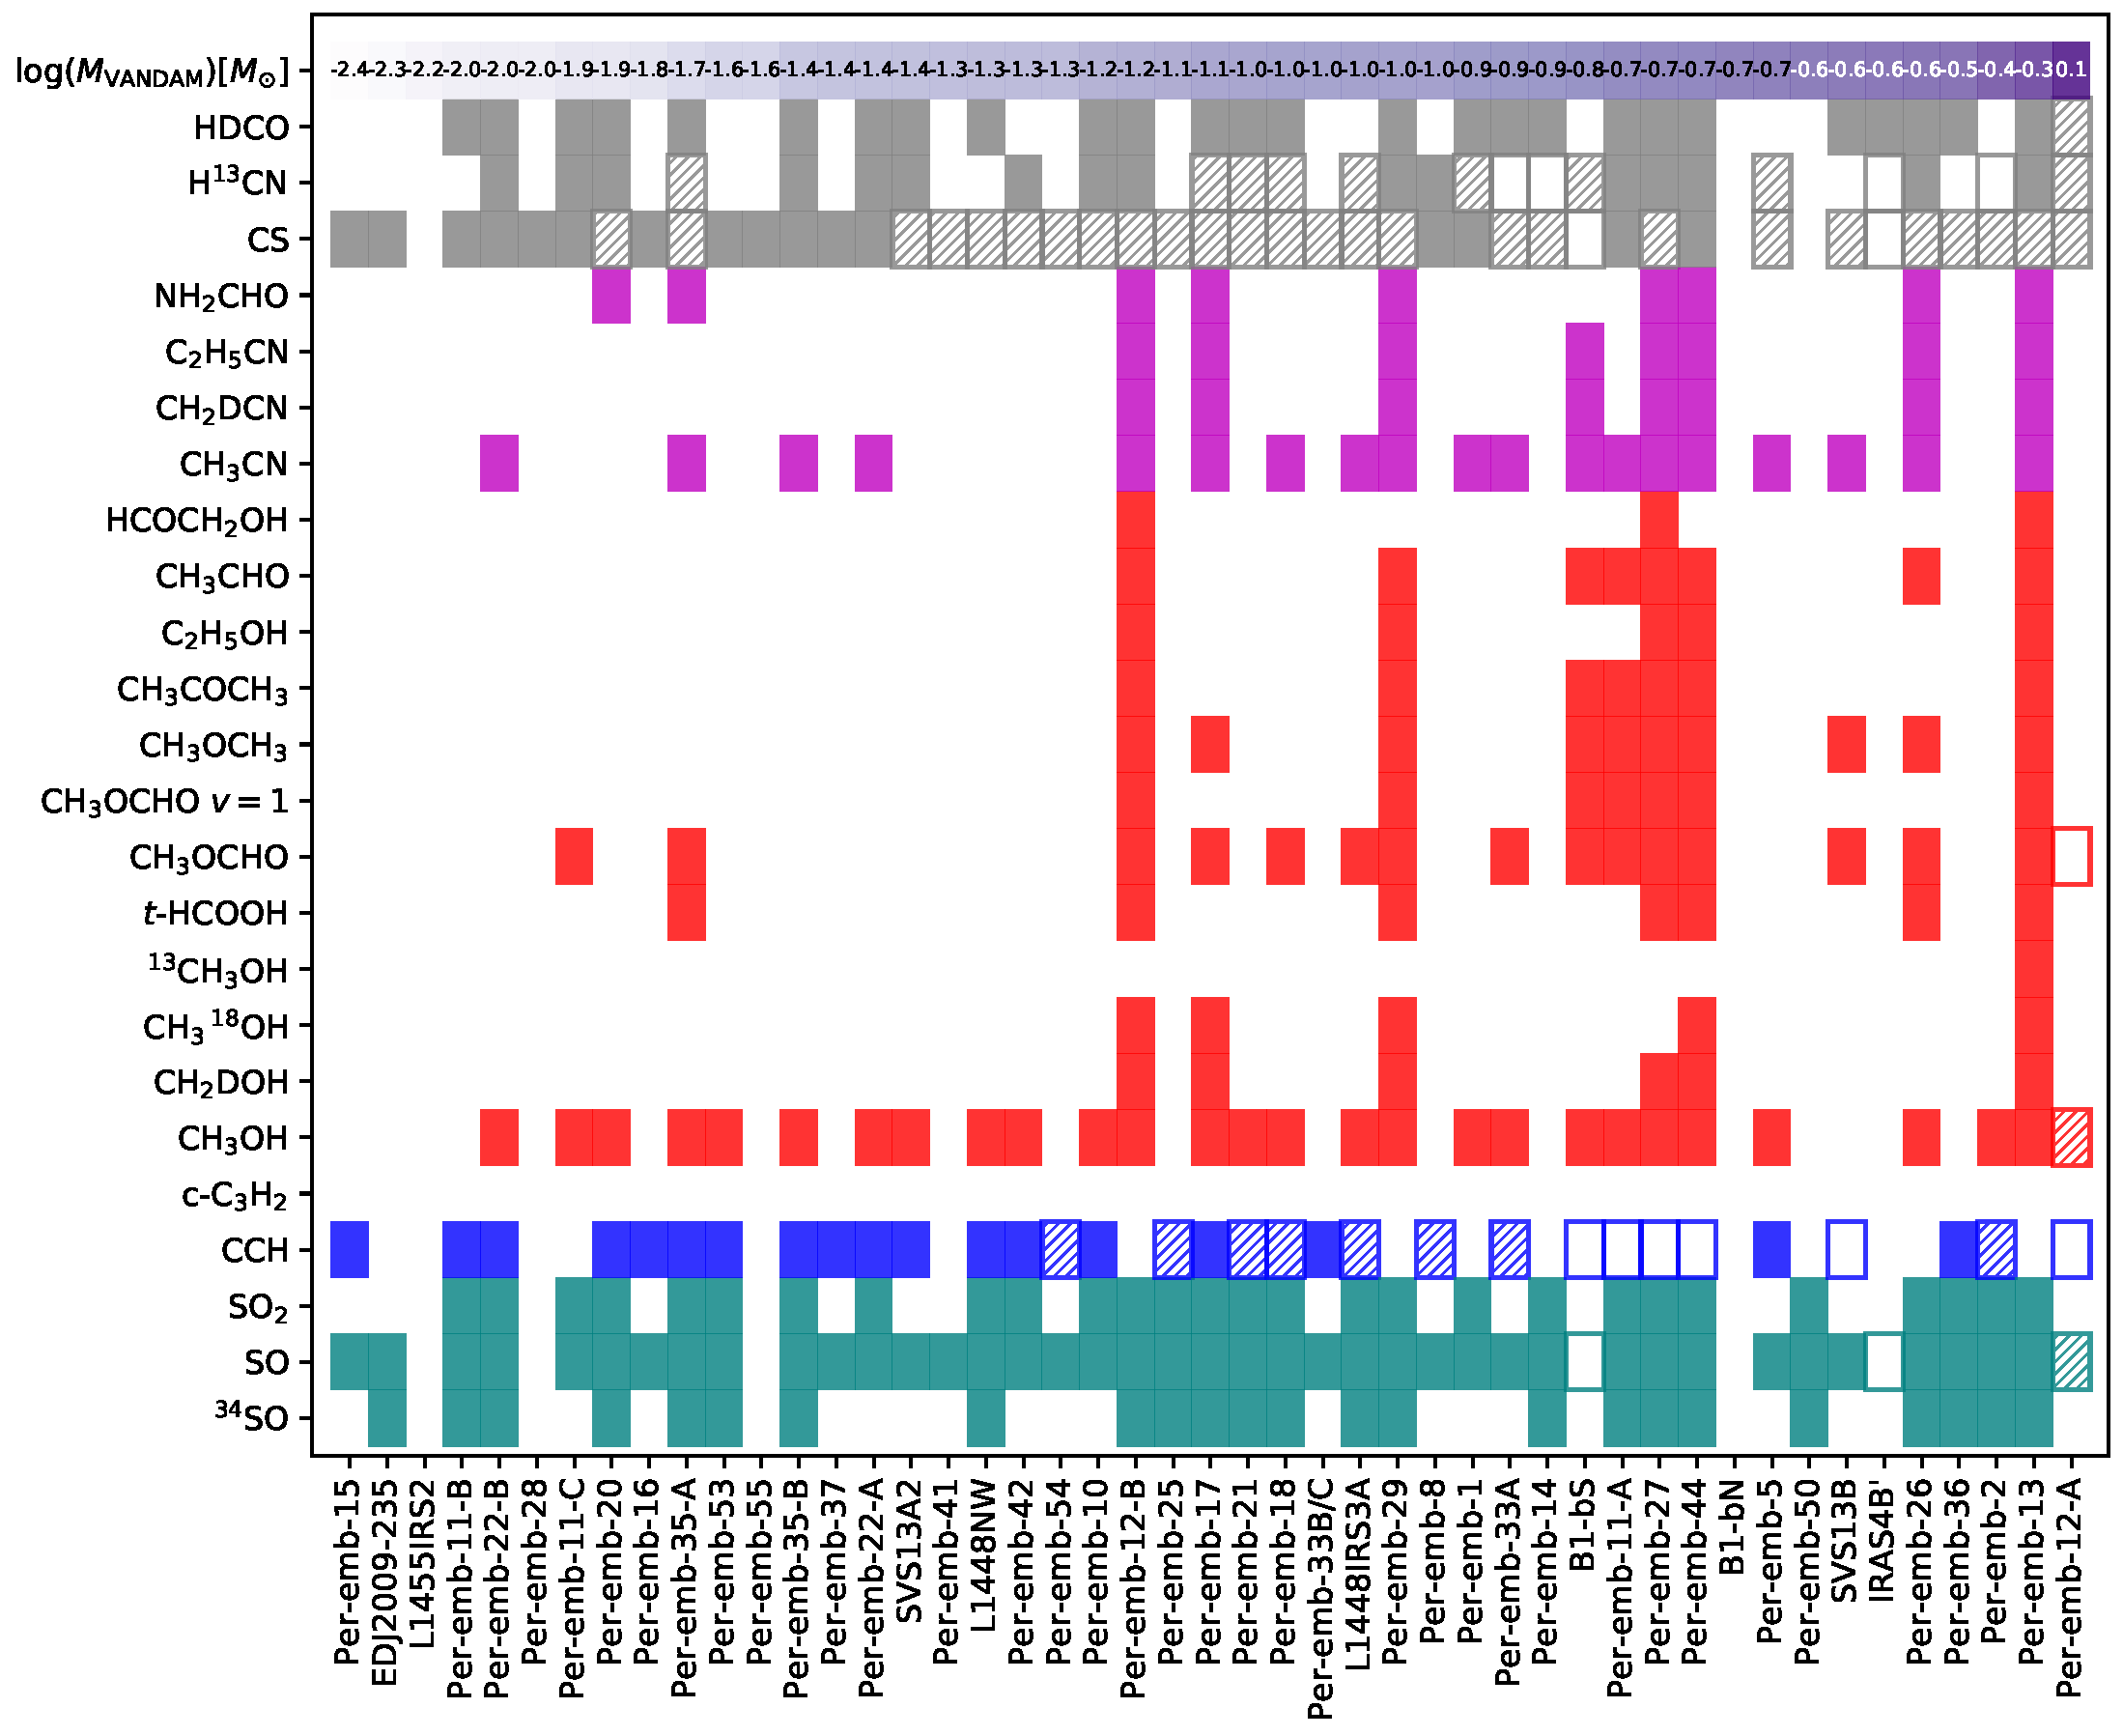
\includegraphics[width=\textwidth]{stats_sorted_by_Mcont.pdf}
  \caption{The same figure as Figure\,\ref{fig:stats} but sorted by their mass derived from their 9\,mm observations \citep{2018ApJS..238...19T}.}
\end{figure*}
\renewcommand{\thefigure}{\arabic{figure}}

\section{Correlations of COMs}
The chemical evolution of protostars may leave certain patterns in the abundance of molecules as the dynamical evolution determines the density and temperature structures, regulating chemical reactions.  Thus, the abundance of COMs and their correlations provide critical information to constrain the chemical evolution at embedded protostars.  The fitted column density of COMs indicates the abundance of COMs around protostars.  Typically COMs are locked into the ices on dust grains at outer envelope.  \textcolor{red}{The formation of COMs at diffuse clouds relies on non-thermal process, such as cosmic rays, whose contribution is negligible compared to the central warm region.}  Therefore, we take the column density of COMs as a proxy of the abundance of COMs.  

As described in Section\,\ref{sec:modeling}, we fit the column density and line width with different excitation temperatures, which result in a range of column density as its uncertainty.  The comparison between CCH and \methanol\ shows no correlation between these two molecules (Figure\,\ref{fig:cch_ch3oh}), similar to the conclusion in \citet{2018ApJS..236...52H}.  The single dish survey by \citet{2016ApJ...833..125G} shows a correlation between C$_{4}$H, a more complex carbon-chain molecules, and \methanol.  Outflow activity can promote the formation of CCH, which is more efficiency at warm temperature.  In face, the morphology of CCH often traces the outflow cavities seen from CS.  Therefore, the lack of correlation between CCH and \methanol\ may be affected by outflows.

Figure\,\ref{fig:corner} shows the correlations of several COMs selected from their detection rates.  The column density of \methanol\ best correlates with that of \methylcyanide.  \citet{2020A&A...635A.198B} also found the tight correlation between these two molecules.  

Similar column densities of \methylformate\ and \dimethylether\ indicate a tight correlation


\begin{figure}[htbp!]
  \centering
  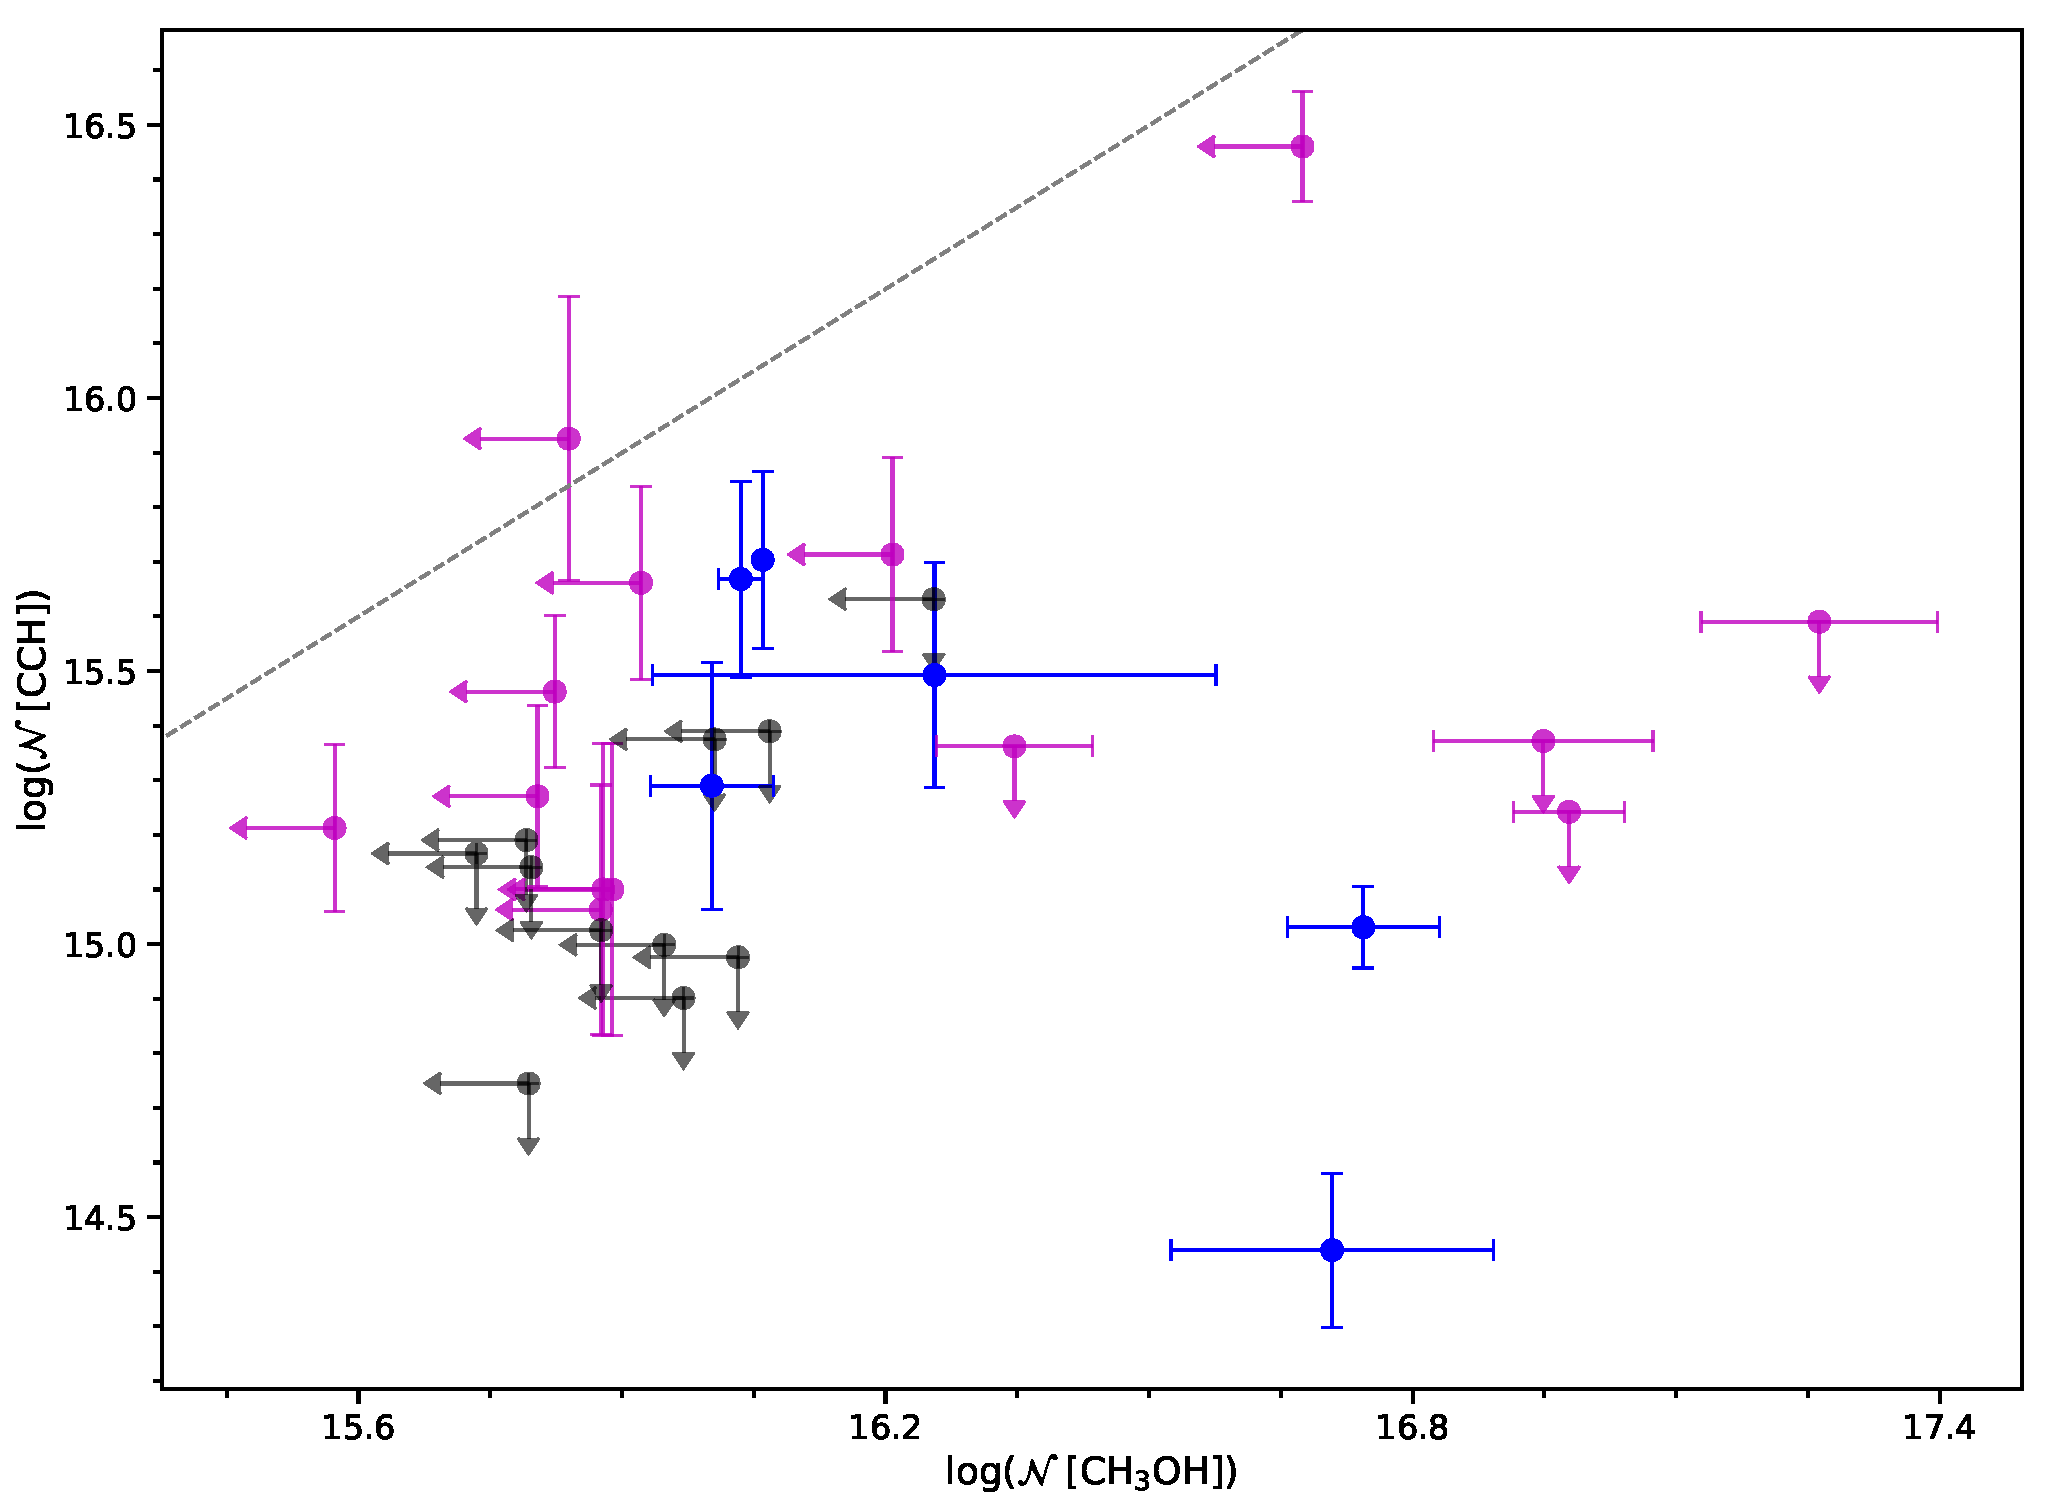
\includegraphics[width=0.47\textwidth]{Ncol_ch3oh_cch.pdf}
  \caption{Correlation of the column densities of CCH and \methanol\ fitted from the PEACHES protostars.  The sources where both molecules are detected are shown in black; the sources where only one molecule is detected are shown in magenta; finally, the sources where both molecules are not detected are shown in black for the corresponding upper limits.}
  \label{fig:cch_ch3oh}
\end{figure}

\begin{figure*}[htbp!]
  \centering
  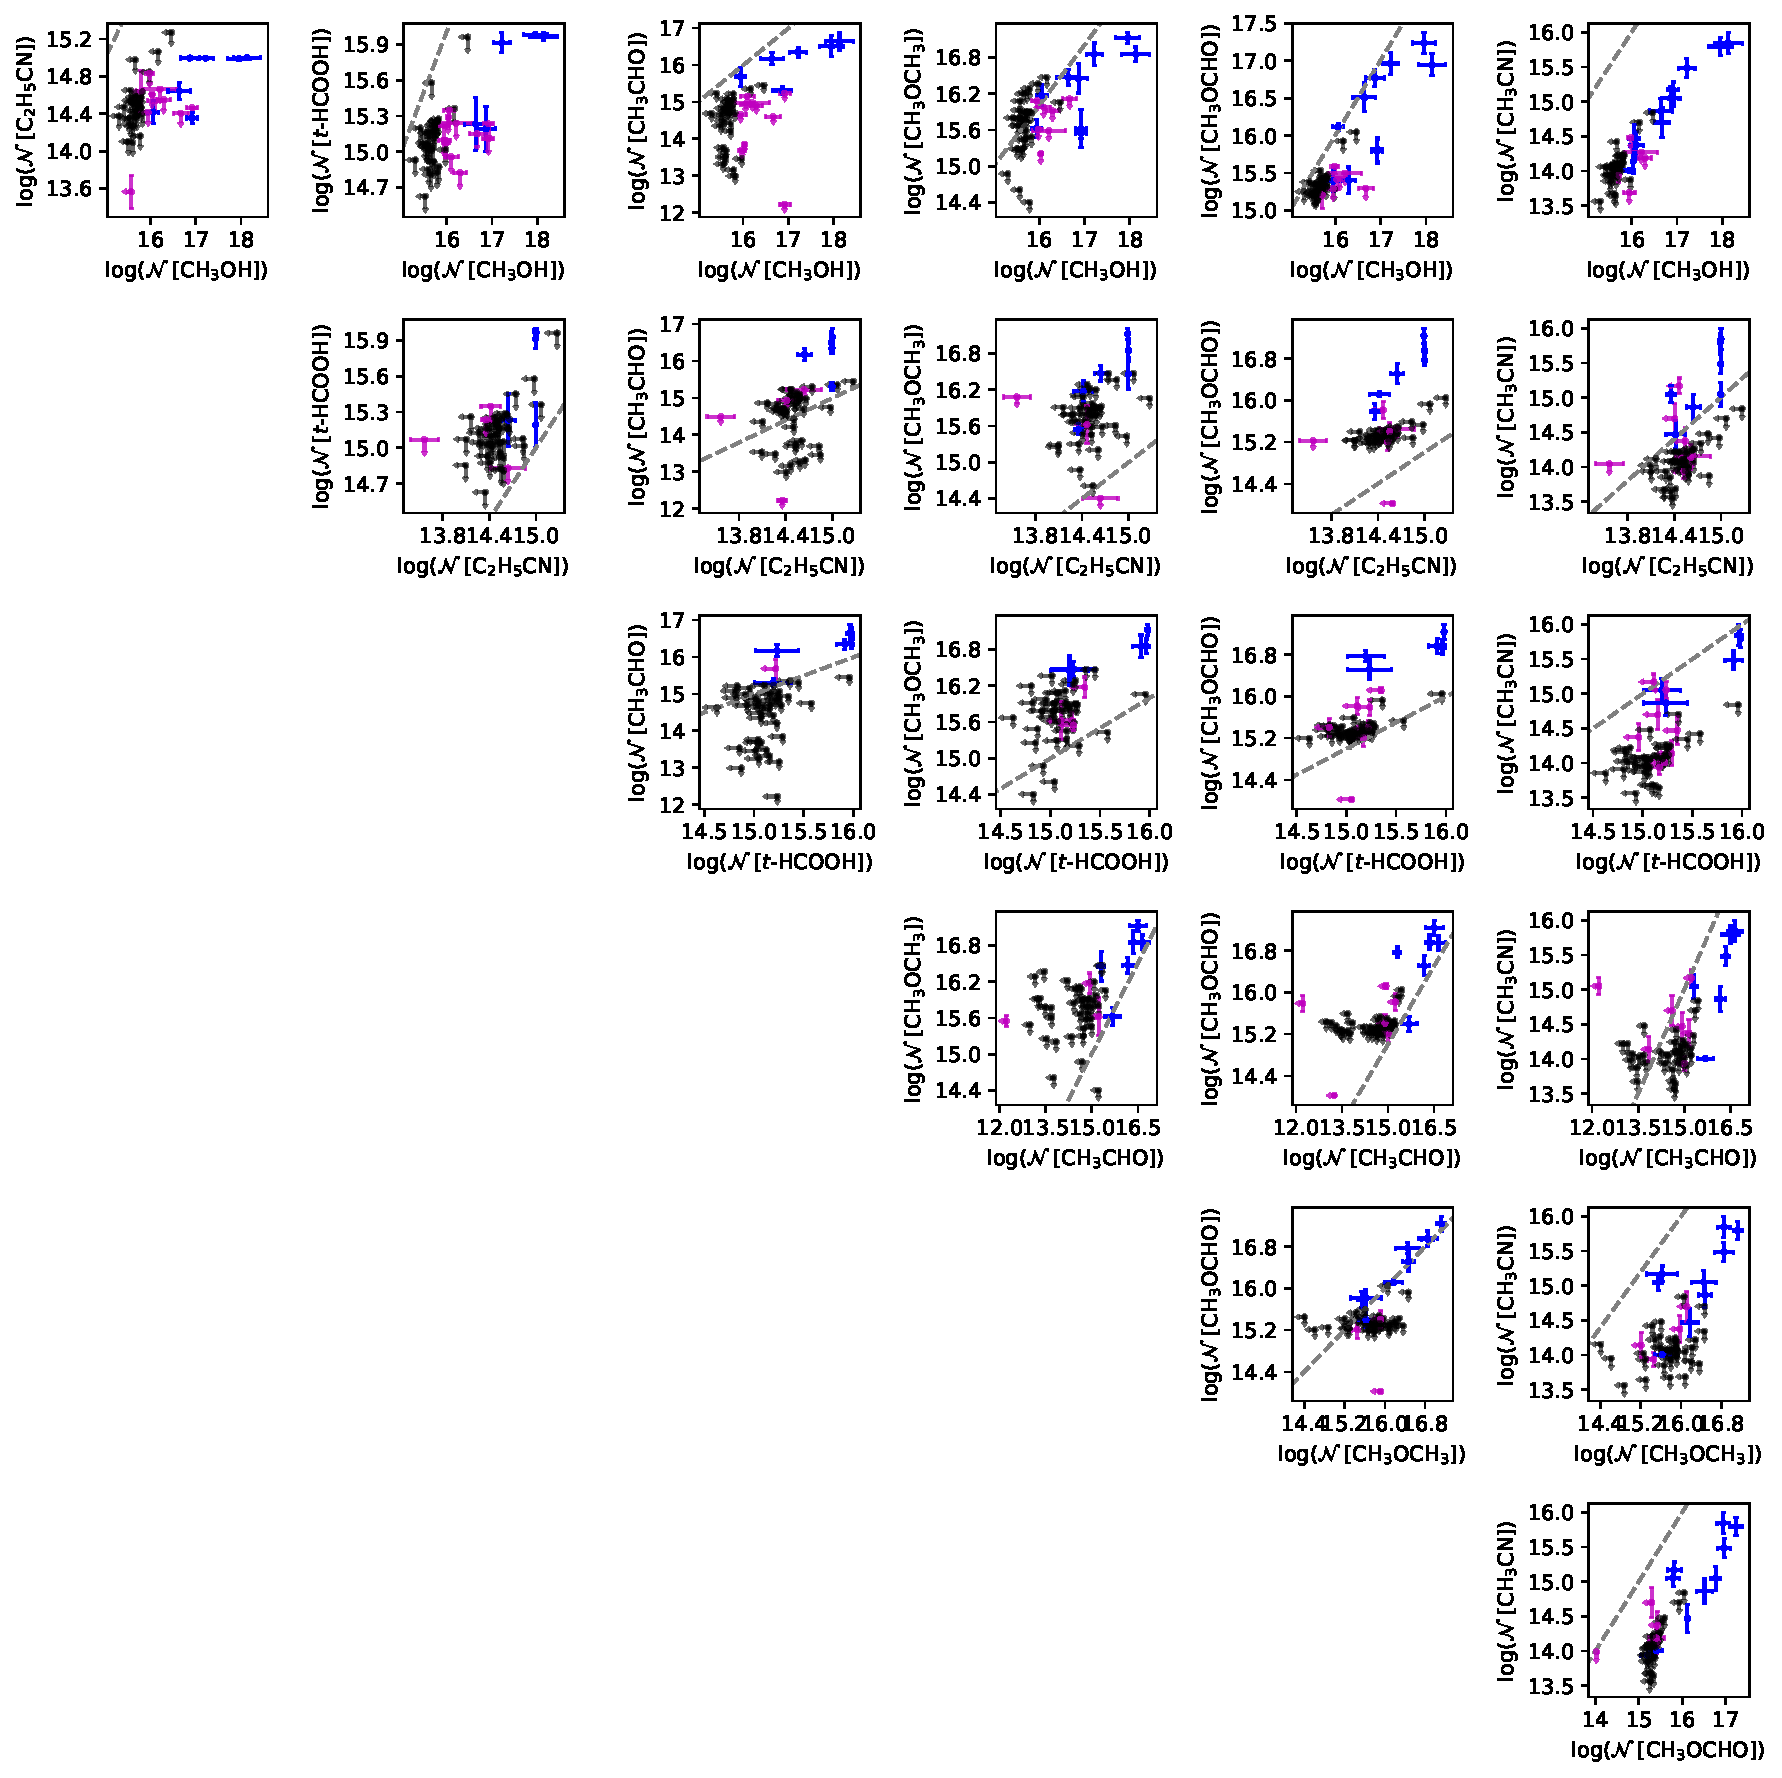
\includegraphics[width=\textwidth]{corner_Ncol.pdf}
  \caption{Corner plot of the correlations of the column densities between \methanol, \methylcyanide, \methylformate, \dimethylether, \acetaldehyde, \ethylcyanide, and $t$-HCOOH.  The color code follows that in Figure\,\ref{fig:ccg_ch3oh}.  The dashed line indicates equality.}
  \label{fig:corner}
\end{figure*}

\section{Spatial Extent of COMs}
\section{Discussion}
\subsection{Complex Chemistry throughout Star Formation}

% \subsection{Source Velocities}
% From the \sosigma\ lines at 258255.8259\,MHz and 261843.7210\,MHz along with the CS \jj{5}{4} line, the averaged source velocities of Per-emb-37 and EDJ2009-172 are 7.437$\pm$0.056\kms\ and 7.748$\pm$0.212\kms, respectively.  The same two \sosigma\ lines also suggest a source velocity of 6.575$\pm$0.060\kms\ for Per-emb-36.

% \begin{table*}
%   \centering
%   \caption{The source velocities of PEACHES sources}
%   \label{tbl:vlsr}
%   \begin{tabular}{ccccc}
%       \toprule
%       Source      & Species   & Frequency [MHz] & Line FWHM [km s$^{-1}$] \\
%       \midrule
%       Set1\_ID01  & SO        & 258255.8        & 5.06$\pm$1.08           \\
%       Set1\_ID01  & HDCO      & 246925.3        & 3.03$\pm$1.58           \\
%       Set2\_ID03  & \methanol & 261805.7        & 3.44$\pm$0.02           \\
%       \bottomrule
%   \end{tabular}
% \end{table*}

\subsection{1D Spectra}

% \begin{deluxetable*}{ccccc}
    \tabletypesize{\scriptsize}
    \tablecaption{Line width fitting \label{tbl:line_width}}
    \tablewidth{\textwidth}
    \tablehead{\colhead{Line} & \colhead{$\nu_\text{rest}$} & \colhead{$\nu_\text{line}$} & 
    \colhead{T$_\text{peak}$} & \colhead{$\Delta\,v$} \\ 
    \colhead{} & \colhead{(MHz)} & \colhead{(MHz)} & \colhead{(K)} & \colhead{(km s$^{-1}$)}}
    \startdata
    \multicolumn{5}{c}{Per-emb-22-B} \\ % Set1_ID03_2
    \hline
    \methanol       & 243915.79 & 243915.39$\pm$0.20 & 1.31$\pm$0.13    & 2.13$\pm$0.25 \\
    SO$_{2}$        & 244254.22 & 244254.06$\pm$0.23 & 1.14$\pm$0.15    & 1.85$\pm$0.29 \\
    \multicolumn{5}{c}{Per-emb-22-A} \\
    \hline
    \multicolumn{5}{c}{L1448NW} \\
    \hline
    \multicolumn{5}{c}{Per-emb-33B/C} \\
    \hline
    \multicolumn{5}{c}{Per-emb-33} \\
    \hline
    \multicolumn{5}{c}{Per-emb-33A} \\
    \hline
    \multicolumn{5}{c}{L1448\,IRS3A} \\
    \hline
    \multicolumn{5}{c}{Per-emb-26} \\
    \hline
    \multicolumn{5}{c}{Per-emb-42} \\
    \hline
    \multicolumn{5}{c}{Per-emb-25} \\
    \hline
    \multicolumn{5}{c}{Per-emb-17} \\
    \hline
    \multicolumn{5}{c}{Per-emb-20} \\
    \hline
    \multicolumn{5}{c}{L1455\,IRS2} \\
    \hline
    \multicolumn{5}{c}{Per-emb-35-A} \\
    \hline
    \multicolumn{5}{c}{Per-emb-35-B} \\
    \hline
    \multicolumn{5}{c}{Per-emb-27} \\
    \hline
    \multicolumn{5}{c}{EDJ2009-172} \\
    \hline
    \multicolumn{5}{c}{Per-emb-36} \\
    \hline
    \multicolumn{5}{c}{Per-emb-54} \\
    \hline
    \multicolumn{5}{c}{SVS13B} \\
    \hline
    \multicolumn{5}{c}{SVS13A2} \\
    \hline
    \multicolumn{5}{c}{Per-emb-44} \\
    \hline
    \multicolumn{5}{c}{Per-emb-15} \\
    \hline
    \multicolumn{5}{c}{Per-emb-50} \\
    \hline
    \multicolumn{5}{c}{Per-emb-12-B} \\
    \hline
    \multicolumn{5}{c}{Per-emb-12-A} \\
    \hline
    \multicolumn{5}{c}{Per-emb-21} \\
    \hline
    \multicolumn{5}{c}{Per-emb-18} \\
    \hline
    \multicolumn{5}{c}{Per-emb-13} \\
    \hline
    \multicolumn{5}{c}{IRAS4B'} \\
    \hline
    \multicolumn{5}{c}{Per-emb-14} \\
    \hline
    \multicolumn{5}{c}{EDJ2009-235} \\
    \hline
    \multicolumn{5}{c}{Per-emb-37} \\
    \hline
    \multicolumn{5}{c}{Per-emb-60} \\
    \hline
    \multicolumn{5}{c}{Per-emb-5} \\
    \hline
    \multicolumn{5}{c}{Per-emb-2} \\
    \hline
    \multicolumn{5}{c}{Per-emb-10} \\
    \hline
    \multicolumn{5}{c}{Per-emb-40} \\
    \hline
    \multicolumn{5}{c}{Per-emb-29} \\
    \hline
    \multicolumn{5}{c}{B1-bN} \\
    \hline
    \multicolumn{5}{c}{B1-bS} \\
    \hline
    \multicolumn{5}{c}{Per-emb-16} \\
    \hline
    \multicolumn{5}{c}{Per-emb-28} \\
    \hline
    \multicolumn{5}{c}{Per-emb-1} \\
    \hline
    \multicolumn{5}{c}{Per-emb-11-B} \\
    \hline
    \multicolumn{5}{c}{Per-emb-11-A} \\
    \hline
    \multicolumn{5}{c}{Per-emb-11-C} \\
    \hline
    \multicolumn{5}{c}{Per-emb-55} \\
    \hline
    \multicolumn{5}{c}{Per-emb-8} \\
    \hline
    \multicolumn{5}{c}{Per-emb-53} \\
    \hline
    \enddata
\end{deluxetable*}

% \section{Analyses}
% Line identification
% The derivation of column density
% - XCLASS fitting
% - the caveats of the XCLASS fitting
%   - the assumption of a Gaussian profile: self absorption, non-Gaussian lines
% - MCMC fitting for methyl formate

% The correlation of column densities

% The morphology of COMs



% \subsection{The Correlations of Column Densities}
% \begin{deluxetable*}{ccccccc}
    \tabletypesize{\scriptsize}
    \tablecaption{MCMC Fitting of Methyl Formate \label{tbl:mf_temp}}
    \tablewidth{\textwidth}
    \tablehead{\colhead{Source} & \multicolumn{2}{c}{Temperature [K]} & 
               \multicolumn{2}{c}{log($\mathcal{N}$) [cm$^{-2}$]} & \multicolumn{2}{c}{Line width [km s$^{-1}$]} \\
               \colhead{} & \colhead{best} & \colhead{mode$\pm$HPD} &
               \colhead{best} & \colhead{mode$\pm$HPD} &
               \colhead{best} & \colhead{mode$\pm$HPD}}
    
    \startdata
    Set1\_ID01\_2 & 95 & 76$^{+315}_{-56}$ & 15.24 & 15.29$^{+0.42}_{-0.42}$ & 4.86 & 4.77$^{+0.22}_{-0.52}$ \\
    Set1\_ID01 & 980 & 995$^{+5}_{-89}$ & 15.76 & 15.28$^{+0.57}_{-0.57}$ & 3.51 & 3.51$^{+1.45}_{-1.07}$ \\
    Set1\_ID02 & 87 & 98$^{+14}_{-41}$ & 15.67 & 15.67$^{+0.10}_{-0.08}$ & 3.66 & 4.06$^{+0.65}_{-0.79}$ \\
    Set1\_ID06 & 93 & 93$^{+59}_{-35}$ & 15.67 & 15.67$^{+0.12}_{-0.08}$ & 4.84 & 4.77$^{+0.22}_{-0.02}$ \\
    Set2\_ID00 & 263 & 310$^{+3}_{-56}$ & 16.89 & 16.92$^{+0.05}_{-0.04}$ & 3.95 & 3.95$^{+0.15}_{-0.12}$ \\
    Set2\_ID01\_2 & 217 & 194$^{+75}_{-4}$ & 16.37 & 16.36$^{+0.10}_{-0.03}$ & 2.22 & 2.25$^{+0.14}_{-0.12}$ \\
    Set2\_ID02 & 195 & 225$^{+119}_{-64}$ & 16.04 & 16.10$^{+0.20}_{-0.09}$ & 1.21 & 1.21$^{+0.00}_{-0.01}$ \\
    Set2\_ID03 & 931 & 988$^{+11}_{-99}$ & 17.29 & 17.31$^{+0.01}_{-0.05}$ & 4.97 & 4.97$^{+0.03}_{-0.01}$ \\
    Set2\_ID05 & 830 & 792$^{+207}_{-138}$ & 15.70 & 15.70$^{+0.23}_{-0.73}$ & 1.97 & 1.53$^{+0.98}_{-0.33}$ \\
    Set2\_ID07 & 152 & 131$^{+281}_{-120}$ & 14.79 & 14.72$^{+0.53}_{-0.43}$ & 3.24 & 1.66$^{+2.26}_{-0.40}$ \\
    Set2\_ID08 & 159 & 10$^{+551}_{-0}$ & 14.75 & 14.11$^{+0.85}_{-0.04}$ & 2.37 & 1.20$^{+2.15}_{-0.00}$ \\
    Set2\_ID12 & 115 & 41$^{+269}_{-30}$ & 14.96 & 15.02$^{+0.05}_{-0.94}$ & 4.54 & 4.89$^{+0.09}_{-1.70}$ \\
    Set3\_ID00 & 98 & 58$^{+41}_{-14}$ & 15.85 & 15.82$^{+0.26}_{-0.09}$ & 1.24 & 1.25$^{+0.02}_{-0.05}$ \\
    Set3\_ID01 & 134 & 134$^{+13}_{-27}$ & 16.59 & 16.60$^{+0.02}_{-0.02}$ & 3.04 & 3.08$^{+0.18}_{-0.15}$ \\
    Set3\_ID07\_3 & 772 & 954$^{+45}_{-404}$ & 15.21 & 15.10$^{+0.05}_{-0.99}$ & 1.21 & 1.21$^{+0.06}_{-0.01}$ \\
    Set3\_ID07 & 104 & 92$^{+182}_{-45}$ & 15.67 & 15.67$^{+0.29}_{-0.15}$ & 2.44 & 2.33$^{+1.22}_{-0.66}$ \\
    \enddata
\end{deluxetable*}


\acknowledgements
Y.-L. Yang acknowledges the supports the JSPS Postdoctoral Fellowship from Japan Society for the Promotion of Science.  This paper makes use of the following ALMA data: ADS/JAO.ALMA\#2016.0.00391.S. ALMA is a partnership of ESO (representing its member states), NSF (USA) and NINS (Japan), together with NRC (Canada), MOST and ASIAA (Taiwan), and KASI (Republic of Korea), in cooperation with the Republic of Chile. The Joint ALMA Observatory is operated by ESO, AUI/NRAO and NAOJ.  The National Radio Astronomy Observatory is a facility of the National Science Foundation operated under cooperative agreement by Associated Universities, Inc.

\facilities{ALMA}

\software{astropy, XCLASS, spectral-cube, CASA}

\appendix
\section{Catalogs for Molecular Data}
\label{sec:catalogs}

\bibliography{research,fixed}

\end{document}
